\documentclass[
  12pt,
  a4paper,
  oneside
]{report}

% Configuração de codificação e idioma (Universal: funciona com pdflatex, xelatex e lualatex)
\usepackage[utf8]{inputenc}
\usepackage[T1]{fontenc}
\usepackage[brazilian]{babel}

% Geometria da página segundo normas ABNT/USP
\usepackage[
  a4paper,
  top=3cm,
  bottom=2cm,
  left=3cm,
  right=2cm
]{geometry}

% Pacotes matemáticos essenciais
\usepackage{amsmath}
\usepackage{amssymb}
\usepackage{amsfonts}
\usepackage{bm}

% Tipografia e Espaçamento
\usepackage{lmodern}
\usepackage{setspace}
\onehalfspacing
\usepackage{microtype}
\usepackage{indentfirst}
\setlength{\parindent}{1.5cm}

% Figuras, Gráficos e Tabelas
\usepackage{graphicx}
\usepackage{booktabs}
\usepackage{tabularx}
\usepackage{longtable}
\usepackage{caption}
\usepackage{subcaption}
\usepackage{enumitem}

% Links e Referências Cruzadas
\usepackage[
  colorlinks=true,
  linkcolor=blue!70!black,
  citecolor=blue!70!black,
  urlcolor=blue!70!black
]{hyperref}
\usepackage[nameinlink,noabbrev,brazilian]{cleveref}

% Formatação dos Títulos de Capítulos
\usepackage{titlesec}
\titleformat{\chapter}[hang]
  {\normalfont\Large\bfseries}
  {\thechapter}
  {1em}
  {\MakeUppercase}
\titleformat{\section}
  {\normalfont\large\bfseries}
  {\thesection}
  {1em}
  {}
\titleformat{\subsection}
  {\normalfont\normalsize\bfseries}
  {\thesubsection}
  {1em}
  {}

% Cabeçalhos e Rodapés
\usepackage{fancyhdr}
\pagestyle{fancy}
\fancyhf{}
\fancyhead[R]{\thepage}
\renewcommand{\headrulewidth}{0pt}

% Informações Institucionais e do Trabalho
\newcommand{\tccuniversidade}{UNIVERSIDADE DE SÃO PAULO}
\newcommand{\tccinstituto}{INSTITUTO DE FÍSICA}
\newcommand{\tccdepartamento}{DEPARTAMENTO DE FÍSICA NUCLEAR}
\newcommand{\tcccurso}{CURSO DE BACHARELADO EM FÍSICA COM HABILITAÇÃO EM FÍSICA MÉDICA}
\newcommand{\tccautor}{WAGNER H. M.}
\newcommand{\tcctitulo}{MODELOS PERCEPTIVOS NA AVALIAÇÃO DA QUALIDADE DE IMAGEM EM TOMOGRAFIA COMPUTADORIZADA: DA TEORIA CLÁSSICA DE DETECÇÃO DE SINAIS AOS MODELOS DE APRENDIZADO PROFUNDO E OTIMIZAÇÃO MULTIOBJETIVO}
\newcommand{\tccorientador}{Prof. Dr. Paulo Roberto Costa}
\newcommand{\tccarea}{Física Médica e Radiológica}
\newcommand{\tcccidade}{SÃO PAULO}
\newcommand{\tccano}{2026}

\begin{document}

% ==============================================================================
% ELEMENTOS PRÉ-TEXTUAIS
% ==============================================================================
\pagestyle{empty}

% 1. CAPA
\begin{center}
  {\bfseries\large \tccuniversidade \par}
  {\bfseries\large \tccinstituto \par}
  {\bfseries\large \tccdepartamento \par}
  {\bfseries\normalsize \tcccurso \par}

  \vspace{3.5cm}

  {\bfseries\Large \tccautor \par}

  \vspace{3.5cm}

  {\bfseries\large \tcctitulo \par}

  \vfill

  {\bfseries\large \tcccidade \par}
  {\bfseries\large \tccano \par}
\end{center}
\clearpage

% 2. FOLHA DE ROSTO
\begin{center}
  {\bfseries\Large \tccautor \par}

  \vspace{3.5cm}

  {\bfseries\large \tcctitulo \par}

  \vspace{2.5cm}

  \begin{flushright}
    \begin{minipage}{0.55\textwidth}
      \small
      Monografia de Conclusão de Curso apresentada ao Instituto de Física da Universidade de São Paulo, como parte dos requisitos necessários para a obtenção do título de Bacharel em Física com Habilitação em Física Médica.
      
      \vspace{0.5cm}
      \textbf{Orientador:} \tccorientador\\
      \textbf{Área de Concentração:} \tccarea
    \end{minipage}
  \end{flushright}

  \vfill

  {\bfseries\large \tcccidade \par}
  {\bfseries\large \tccano \par}
\end{center}
\clearpage

% 3. FOLHA DE APROVAÇÃO
\begin{center}
  {\bfseries\Large FOLHA DE APROVAÇÃO \par}
  
  \vspace{1.5cm}
  
  {\bfseries\large \tccautor \par}
  
  \vspace{0.8cm}
  
  {\bfseries \tcctitulo \par}

  \vspace{1.5cm}

  \begin{flushright}
    \begin{minipage}{0.55\textwidth}
      \small
      Monografia de Conclusão de Curso defendida e aprovada em \underline{\hspace{1cm}} de \underline{\hspace{3.5cm}} de \tccano{} pela banca examinadora constituída pelos seguintes membros:
    \end{minipage}
  \end{flushright}

  \vspace{1.8cm}

  \rule{0.85\textwidth}{0.5pt}\\
  \textbf{\tccorientador{} (Orientador / Presidente)}\\
  Instituto de Física da Universidade de São Paulo -- IFUSP

  \vspace{1.2cm}

  \rule{0.85\textwidth}{0.5pt}\\
  \textbf{Membro da Banca Examinadora 1}\\
  Instituto de Radiologia do Hospital das Clínicas -- InRad-HCFMUSP

  \vspace{1.2cm}

  \rule{0.85\textwidth}{0.5pt}\\
  \textbf{Membro da Banca Examinadora 2}\\
  Instituto de Física da Universidade de São Paulo -- IFUSP
\end{center}
\clearpage

% 4. RESUMO
\chapter*{Resumo}
\addcontentsline{toc}{chapter}{Resumo}

A Tomografia Computadorizada (TC) desempenha papel indispensável na medicina diagnóstica moderna, operando sob o permanente compromisso físico entre a minimização da dose de radiação ionizante e a preservação do desempenho diagnóstico (princípio ALARA). Historicamente, a metrologia e a garantia da qualidade em TC apoiaram-se em grandezas físicas escalares e lineares, como a Relação Sinal-Ruído (SNR), a Relação Contraste-Ruído (CNR) e a Função de Transferência de Modulação (MTF), avaliadas em simuladores geométricos homogêneos. No entanto, a incorporação clínica de algoritmos avançados não lineares --- com destaque para as reconstruções iterativas estatísticas e, fundamentalmente, as reconstruções baseadas em aprendizado profundo (\emph{Deep Learning Image Reconstruction} --- DLR) --- quebrou as premissas de linearidade e invariância translacional do sistema formador de imagens. Sob processamentos não lineares, o ruído tomográfico tornou-se espacialmente heterogêneo, dependente da dose, do contraste e da geometria local da cena, induzindo alterações texturais perceptuais (como a textura cerosa ou \emph{plastic/waxy look}) que não são capturadas pelas métricas clássicas. Para superar essa limitação, a física médica consolidou o paradigma da Qualidade de Imagem Baseada em Tarefa (\emph{Task-Based Image Quality} --- TBIQ), ancorado na Teoria de Detecção de Sinais (\emph{Signal Detection Theory} --- SDT), no qual a qualidade da imagem é formalmente definida pelo desempenho de um observador (humano ou computacional) na execução de uma tarefa diagnóstica clínica específica, quantificada pelo Índice de Detectabilidade ($d'$). Este trabalho apresenta uma investigação exaustiva e estruturada da evolução dos observadores de modelo (\emph{model observers}). Analisa-se a transição histórica do Observador Ideal Bayesiano para os modelos lineares antropomórficos com filtro ocular (NPWE) e canais corticais de frequência (CHO), demonstrando suas deduções matemáticas contínuas no domínio de Fourier e evidenciando os limites biofísicos que causam seu colapso sob reconstruções DLR e fundos anatômicos complexos. Em resposta, investiga-se a fronteira científica representada pelos Observadores Baseados em Aprendizado Profundo (\emph{Deep Learning Model Observers} --- DLMO), baseados em arquiteturas \emph{Vision Transformers} (ViT) com mecanismos de auto-atenção multi-cabeça, calibrados diretamente contra leituras psicofísicas de radiologistas em experimentos de Escolha Forçada entre Duas Alternativas (2AFC) sob análise estatística \emph{Multi-Reader Multi-Case} (MRMC). Detalham-se a física dos detectores de contagem de fótons (PCCT), a síntese de Imagens Monoenergéticas Virtuais ($VMI$) e a formulação da Otimização Multiobjetivo através da Fronteira de Pareto Tridimensional $(D, T, -W)$, que integra dose de radiação ($D$), tempo operacional total ($T$) e detectabilidade ($W$). Esta monografia consolida as bases teóricas, biofísicas e metrológicas que sustentam a pesquisa de Doutorado Direto do autor no IFUSP.

\vspace{0.8cm}
\noindent\textbf{Palavras-chave:} Tomografia Computadorizada. Qualidade de Imagem Baseada em Tarefa. Observadores de Modelo. Índice de Detectabilidade. Reconstrução por Aprendizado Profundo. Vision Transformers. Tomografia por Contagem de Fótons. ANOVA MRMC. Simuladores Antropomórficos. Otimização Multiobjetivo. Fronteira de Pareto.
\clearpage

% 5. ABSTRACT
\chapter*{Abstract}
\addcontentsline{toc}{chapter}{Abstract}

Computed Tomography (CT) plays an indispensable role in modern diagnostic medicine, permanently operating under the physical trade-off between minimizing ionizing radiation dose and preserving diagnostic efficacy (the ALARA principle). Historically, image quality assurance in CT relied on linear scalar metrics, such as Signal-to-Noise Ratio (SNR), Contrast-to-Noise Ratio (CNR), and Modulation Transfer Function (MTF), evaluated on homogeneous geometric phantoms. However, the clinical adoption of advanced non-linear reconstruction algorithms---including iterative reconstructions and Deep Learning Image Reconstruction (DLR)---has broken the foundational assumptions of system linearity and shift-invariance. Under non-linear processing, image noise becomes spatially non-stationary, dose-dependent, and scene-dependent, introducing perceptual texture alterations (such as the ``plastic'' or ``waxy'' appearance) that cannot be properly captured by conventional scalar metrics. To overcome this metrological limitation, medical physics has consolidated the Task-Based Image Quality (TBIQ) paradigm, grounded in Signal Detection Theory (SDT), where image quality is rigorously defined by the performance of an observer (human radiologist or mathematical model) executing a specific clinical task, quantified by the Detectability Index ($d'$). This monograph provides a comprehensive investigation of the evolution of model observers. We analyze the historical transition from the Bayesian Ideal Observer to anthropomorphic linear models incorporating eye filters (NPWE) and cortical frequency channels (CHO), detailing their continuous mathematical derivations in the Fourier domain and demonstrating their breakdown in non-linear DLR regimes and structured anatomical backgrounds. In response, we investigate the state of the art in Deep Learning Model Observers (DLMO), which leverage self-attention neural architectures (Vision Transformers) calibrated against expert radiologists' psychophysical performance in Two-Alternative Forced Choice (2AFC) paradigms under Multi-Reader Multi-Case (MRMC) statistical modeling. Furthermore, we explore the physics of Photon-Counting CT (PCCT), the synthesis of Virtual Monoenergetic Images (VMI), and the formulation of Multi-Objective Optimization via the Three-Dimensional Pareto Frontier $(D, T, -W)$, which integrates radiation dose ($D$), operational time ($T$), and diagnostic detectability ($W$). This study establishes the theoretical, computational, and physical foundation required for next-generation CT metrology, directly supporting the author's Direct Doctorate research at IFUSP.

\vspace{0.8cm}
\noindent\textbf{Keywords:} Computed Tomography. Task-Based Image Quality. Model Observers. Detectability Index. Deep Learning Reconstruction. Vision Transformers. Photon-Counting CT. ANOVA MRMC. Anthropomorphic Phantoms. Multi-Objective Optimization. Pareto Frontier.
\clearpage

% 6. LISTA DE ILUSTRAÇÕES
\pdfbookmark[0]{\listfigurename}{lof}
\listoffigures
\clearpage

% 7. LISTA DE TABELAS
\pdfbookmark[0]{\listtablename}{lot}
\listoftables
\clearpage

% 8. LISTA DE ABREVIATURAS E SIGLAS
\chapter*{Lista de Abreviaturas e Siglas}
\addcontentsline{toc}{chapter}{Lista de Abreviaturas e Siglas}

\begin{longtable}{ll}
\toprule
\textbf{Sigla} & \textbf{Significado} \\
\midrule
\endhead
\textbf{2AFC} & \emph{Two-Alternative Forced Choice} (Escolha Forçada entre Duas Alternativas) \\
\textbf{AAPM} & \emph{American Association of Physicists in Medicine} \\
\textbf{AEC} & \emph{Automatic Exposure Control} (Controle Automático de Exposição) \\
\textbf{ALARA} & \emph{As Low As Reasonably Achievable} (Tão Baixo Quanto Razoavelmente Exequível) \\
\textbf{ANOVA} & \emph{Analysis of Variance} (Análise de Variância) \\
\textbf{ASiR} & \emph{Adaptive Statistical Iterative Reconstruction} \\
\textbf{AUC} & \emph{Area Under the ROC Curve} (Área sob a Curva ROC) \\
\textbf{BKE} & \emph{Background Known Exactly} (Fundo Conhecido Exatamente) \\
\textbf{BKS} & \emph{Background Known Statistically} (Fundo Conhecido Estatisticamente) \\
\textbf{CBR} & Colégio Brasileiro de Radiologia e Diagnóstico por Imagem \\
\textbf{CdTe} & Telureto de Cádmio (semicondutor de conversão direta) \\
\textbf{CEP} & Comitê de Ética em Pesquisa \\
\textbf{CHO} & \emph{Channelized Hotelling Observer} (Observador de Hotelling Canalizado) \\
\textbf{CNR} & \emph{Contrast-to-Noise Ratio} (Relação Contraste-Ruído) \\
\textbf{CONEP} & Comissão Nacional de Ética em Pesquisa \\
\textbf{CSF} & \emph{Contrast Sensitivity Function} (Função de Sensibilidade ao Contraste) \\
\textbf{CTDI} & \emph{Computed Tomography Dose Index} (Índice de Dose em Tomografia Computadorizada) \\
\textbf{CZT} & Telureto de Cádmio e Zinco \\
\textbf{D-DOG} & \emph{Dense Difference of Gaussians} (Diferença Densa de Gaussianas) \\
\textbf{DBM} & Dorfman-Berbaum-Metz (modelo estatístico para MRMC) \\
\textbf{DLR} & \emph{Deep Learning Image Reconstruction} (Reconstrução por Aprendizado Profundo) \\
\textbf{DLMO} & \emph{Deep Learning Model Observer} (Observador de Modelo por Aprendizado Profundo) \\
\textbf{DLP} & \emph{Dose-Length Product} (Produto Dose-Comprimento) \\
\textbf{DQE} & \emph{Detective Quantum Efficiency} (Eficiência Quântica de Detecção) \\
\textbf{DRL} & \emph{Diagnostic Reference Level} (Nível de Referência Diagnóstica) \\
\textbf{EICT} & \emph{Energy-Integrating Computed Tomography} (TC por Integração de Energia) \\
\textbf{ESF} & \emph{Edge Spread Function} (Função de Resposta ao Degrau) \\
\textbf{FBP} & \emph{Filtered Backprojection} (Retroprojeção Filtrada) \\
\textbf{FOV} & \emph{Field of View} (Campo de Visão) \\
\textbf{GDRFM} & Grupo de Dosimetria e Radioproteção em Física Médica do IFUSP \\
\textbf{GPU} & \emph{Graphics Processing Unit} (Unidade de Processamento Gráfico) \\
\textbf{GSDF} & \emph{Grayscale Standard Display Function} (Função de Exibição Padrão em Tons de Cinza) \\
\textbf{HIR} & \emph{Hybrid Iterative Reconstruction} (Reconstrução Iterativa Híbrida) \\
\textbf{HO} & \emph{Hotelling Observer} (Observador de Hotelling) \\
\textbf{HOR} & Hillis-Obuchowski-Rockette (modelo estatístico de ANOVA MRMC) \\
\textbf{HU} & Unidade Hounsfield (\emph{Hounsfield Unit}) \\
\textbf{IAEA} & \emph{International Atomic Energy Agency} (Agência Internacional de Energia Atômica) \\
\textbf{ICC} & \emph{Intraclass Correlation Coefficient} (Coeficiente de Correlação Intraclasse) \\
\textbf{ICRU} & \emph{International Commission on Radiation Units and Measurements} \\
\textbf{IFUSP} & Instituto de Física da Universidade de São Paulo \\
\textbf{InRad} & Instituto de Radiologia do Hospital das Clínicas da FMUSP \\
\textbf{IO} & \emph{Ideal Observer} (Observador Ideal Bayesiano) \\
\textbf{LG} & Laguerre-Gauss \\
\textbf{LOSO} & \emph{Leave-One-Scanner-Out} (Validação Cruzada Omitindo um Tomógrafo) \\
\textbf{LSF} & \emph{Line Spread Function} (Função de Espalhamento de Linha) \\
\textbf{MBIR} & \emph{Model-Based Iterative Reconstruction} (Reconstrução Iterativa Baseada em Modelos) \\
\textbf{MHSA} & \emph{Multi-Head Self-Attention} (Auto-Atenção Multi-Cabeça) \\
\textbf{MRMC} & \emph{Multi-Reader Multi-Case} (Múltiplos Leitores e Múltiplos Casos) \\
\textbf{MTF} & \emph{Modulation Transfer Function} (Função de Transferência de Modulação) \\
\textbf{NPS} & \emph{Noise Power Spectrum} (Espectro de Potência do Ruído) \\
\textbf{NPW} & \emph{Non-Prewhitening Observer} (Observador Sem Pré-Branqueamento) \\
\textbf{NPWE} & \emph{Non-Prewhitening Observer with Eye Filter} (NPW com Filtro Ocular) \\
\textbf{NSGA-II} & \emph{Non-dominated Sorting Genetic Algorithm II} \\
\textbf{OR} & Obuchowski-Rockette \\
\textbf{PACS} & \emph{Picture Archiving and Communication System} \\
\textbf{PCCT} & \emph{Photon-Counting Computed Tomography} (TC por Contagem de Fótons) \\
\textbf{PSF} & \emph{Point Spread Function} (Função de Resposta ao Ponto) \\
\textbf{ROC} & \emph{Receiver Operating Characteristic} (Característica de Operação do Receptor) \\
\textbf{ROI} & \emph{Region of Interest} (Região de Interesse) \\
\textbf{SDT} & \emph{Signal Detection Theory} (Teoria de Detecção de Sinais) \\
\textbf{SKE} & \emph{Signal Known Exactly} (Sinal Conhecido Exatamente) \\
\textbf{SKS} & \emph{Signal Known Statistically} (Sinal Conhecido Estatisticamente) \\
\textbf{SNR} & \emph{Signal-to-Noise Ratio} (Relação Sinal-Ruído) \\
\textbf{TBIQ} & \emph{Task-Based Image Quality} (Qualidade de Imagem Baseada em Tarefa) \\
\textbf{TC} & Tomografia Computadorizada \\
\textbf{TCLE} & Termo de Consentimento Livre e Esclarecido \\
\textbf{TG-233} & \emph{Task Group 233} da AAPM \\
\textbf{TOPSIS} & \emph{Technique for Order Preference by Similarity to Ideal Solution} \\
\textbf{TTF} & \emph{Task Transfer Function} (Função de Transferência da Tarefa) \\
\textbf{ViT} & \emph{Vision Transformer} \\
\textbf{VMI} & \emph{Virtual Monoenergetic Image} (Imagem Monoenergética Virtual) \\
\textbf{WSS} & \emph{Wide-Sense Stationary} (Estacionário no Sentido Amplo) \\
\bottomrule
\end{longtable}
\clearpage

% 9. LISTA DE SÍMBOLOS
\chapter*{Lista de Símbolos}
\addcontentsline{toc}{chapter}{Lista de Símbolos}

\begin{longtable}{ll}
\toprule
\textbf{Símbolo} & \textbf{Significado Físico / Unidade} \\
\midrule
\endhead
$\mathbf{g}$ & Vetor de dados de imagem discreta ($\mathbb{R}^N$) \\
$\mathbf{s}$ & Vetor determinístico do sinal ou lesão ($\mathbb{R}^N$) \\
$\mathbf{b}$ & Vetor estocástico de ruído e fundo anatômico ($\mathbb{R}^N$) \\
$t$ & Estatística de teste escalar de decisão \\
$t_c$ & Limiar de corte para decisão diagnóstica \\
$d'$ & Índice de detectabilidade (\emph{d-prime}) \\
$d'_{\text{humano}}$ & Índice de detectabilidade experimental medido em leitores humanos \\
$d'_{\text{NPWE}}$ & Índice de detectabilidade calculado pelo modelo NPWE \\
$d'_{\text{CHO}}$ & Índice de detectabilidade calculado pelo modelo CHO \\
$d'_{\text{DL}}$ & Índice de detectabilidade estimado pelo modelo por aprendizado profundo \\
$\mathbf{K}$ & Matriz de autocovariância do ruído ($N \times N$, em $\text{HU}^2$) \\
$\mathbf{K}_{\mathbf{v}}$ & Matriz de autocovariância reduzida no espaço dos canais ($C \times C$) \\
$\mathbf{w}$ & Vetor de pesos ou template linear de filtragem ($\mathbb{R}^N$) \\
$\mathbf{T}$ & Matriz de operadores de canais corticais ($C \times N$) \\
$TTF(f)$ & Função de Transferência da Tarefa na frequência espacial $f$ (adimensional) \\
$f_{50}$ & Frequência espacial correspondente a 50\% de modulação da TTF ($\text{mm}^{-1}$) \\
$f_{10}$ & Frequência espacial correspondente a 10\% de modulação da TTF ($\text{mm}^{-1}$) \\
$NPS(u, v)$ & Espectro de Potência do Ruído bidimensional ($\text{mm}^2$ ou $\text{HU}^2\cdot\text{mm}^2$) \\
$NPS(f)$ & Espectro de Potência do Ruído radial unidimensional ($\text{HU}^2\cdot\text{mm}^2$) \\
$f_{\text{peak}}$ & Frequência espacial de máxima amplitude do espectro de ruído ($\text{mm}^{-1}$) \\
$f_{\text{av}}$ & Frequência espacial média ponderada do espectro de ruído ($\text{mm}^{-1}$) \\
$E(f)$ & Resposta em frequência do filtro ocular humano / CSF (adimensional) \\
$W_{\text{task}}(f)$ & Espectro de Fourier da morfologia da tarefa diagnóstica ($\text{HU}\cdot\text{mm}^2$) \\
$P_C$ & Proporção empírica de acertos no teste 2AFC ($0 \le P_C \le 1$) \\
$\Phi(x)$ & Função de distribuição cumulativa da variável normal padrão \\
$\Phi^{-1}(p)$ & Função quantil (inversa da distribuição cumulativa normal padrão) \\
$\sigma^2$ & Variância estatística do número de CT em uma região homogênea ($\text{HU}^2$) \\
$\sigma_{\text{int}}^2$ & Variância do ruído neural interno do observador biológico ($\text{HU}^2$) \\
$D$ & Dose de radiação absorvida / $\text{CTDI}_{\text{vol}}$ ($\text{mGy}$) \\
$T$ & Tempo operacional total do procedimento ($T = T_{\text{aq}} + T_{\text{rec}}$, em segundos) \\
$W$ & Desempenho na tarefa diagnóstica ($W = d'$) \\
$\Omega$ & Espaço viável de parâmetros do protocolo tomográfico \\
$\Delta C$ & Contraste radiológico central da lesão em relação ao fundo ($\text{HU}$) \\
$R$ & Raio físico da lesão esférica simulada ($\text{mm}$) \\
$J_1(x)$ & Função de Bessel ordinária de primeira espécie e ordem 1 \\
$Q, K, V$ & Matrizes de Consulta (\emph{Query}), Chave (\emph{Key}) e Valor (\emph{Value}) no mecanismo de atenção \\
$d_k$ & Dimensão dos vetores de projeção no módulo de atenção \\
$\mathbf{z}_0$ & Sequência de \emph{patch embeddings} lineares com codificação posicional \\
$\sigma^2_R$ & Componente de variância associada aos leitores humanos na ANOVA MRMC \\
$\sigma^2_C$ & Componente de variância associada aos casos clínicos na ANOVA MRMC \\
$\sigma^2_{RC}$ & Componente de variância da interação leitor $\times$ caso na ANOVA MRMC \\
\bottomrule
\end{longtable}
\clearpage

% 10. SUMÁRIO
\pdfbookmark[0]{\contentsname}{toc}
\tableofcontents
\clearpage

% ==============================================================================
% ELEMENTOS TEXTUAIS (CAPÍTULOS)
% ==============================================================================
\pagestyle{fancy}
\pagenumbering{arabic}
\setcounter{page}{31}

\chapter{Introdução}
\label{chap:introducao}

\section{O Dilema Fundamental da Tomografia Computadorizada: Dose versus Desempenho Clínico}
\label{sec:dilema_dose}

A Tomografia Computadorizada (TC) revolucionou a medicina diagnóstica desde a sua introdução clínica na década de 1970 por Godfrey Hounsfield. Ao permitir a reconstrução tridimensional de secções transversais do corpo humano com elevada diferenciação de densidades de tecidos moles e resolução espacial submilimétrica, a TC consolidou-se como a modalidade de escolha para o estadiamento oncológico, o planejamento cirúrgico e radioterápico, a avaliação de traumas agudos e o rastreamento precoce de doenças pulmonares e vasculares \cite{mccollough2026, seeram2015, bushberg2020}.

Contudo, o princípio físico basilar da formação da imagem tomográfica reside na atenuação exponencial de feixes de raios X transmitidos através do paciente \cite{attix1986}. A absorção e o espalhamento dessa radiação ionizante no tecido biológico provocam ionizações atômicas e quebras de ligações moleculares em estruturas de DNA celular, associando-se a riscos estocásticos de carcinogênese a longo prazo \cite{icrp103_2007}. Consequentemente, embora represente apenas de 10\% a 15\% do total de procedimentos radiológicos executados mundialmente, a TC responde por aproximadamente 65\% a 70\% de toda a dose coletiva de radiação ionizante de origem médica absorvida pela população humana \cite{iaea_5star_2026, mccollough2026}.

Essa assimetria impõe a aplicação rigorosa do princípio fundamental da radioproteção: o princípio ALARA (\emph{As Low As Reasonably Achievable}) \cite{icrp103_2007, anvisa_rdc611_2022, anvisa_in93_2021}. De acordo com essa diretriz, os protocolos tomográficos devem ser continuamente otimizados para operar na menor dose de radiação compatível com o objetivo diagnóstico desejado.

Para compreender a dificuldade física dessa otimização, é necessário analisar como os fótons de raios X se comportam estatisticamente. A detecção de fótons é um processo estocástico regido pela distribuição de Poisson \cite{knoll2010}. Em termos intuitivos, quanto menor o número de fótons emitidos pelo tubo de raios X, maiores são as flutuações estatísticas percentuais registradas pelos detectores. No domínio da imagem reconstruída, essa incerteza manifesta-se visualmente sob a forma de ruído quântico.

A relação matemática fundamental entre o desvio padrão do ruído ($\sigma_{\text{ruído}}$), o número de fótons detectados ($N_{\text{fótons}}$) e o índice de dose volumétrico ($\text{CTDI}_{\text{vol}}$) é expressa por:
\begin{equation}
  \sigma_{\text{ruído}} \propto \frac{1}{\sqrt{N_{\text{fótons}}}} \propto \frac{1}{\sqrt{\text{CTDI}_{\text{vol}}}}
  \label{eq:ruido_dose}
\end{equation}

Em termos práticos, se um físico médico tentar reduzir a dose de radiação pela metade sem alterar a tecnologia do tomógrafo ou o algoritmo de reconstrução, o nível de ruído da imagem aumentará automaticamente em um fator de $\sqrt{2} \approx 1{,}41$ (ou seja, cerca de 41\% de acréscimo de ruído). Esse ruído adicional sobrepõe-se às estruturas anatômicas sutis, reduzindo a capacidade do radiologista de identificar lesões de baixo contraste, como metástases hepáticas incipientes ou pequenos nódulos pulmonares em vidro fosco.

\section{Limitações Estruturais das Métricas Físicas Globais Tradicionais}
\label{sec:limitacoes_metricas}

Durante quatro décadas, o controle de qualidade e a avaliação de desempenho de tomógrafos hospitalares apoiaram-se em grandezas físicas escalares derivadas da teoria de sistemas lineares e invariantes no espaço \cite{barrett_myers_2004}:
\begin{enumerate}[label=\alph*)]
  \item Desvio padrão do número CT ($\sigma_{\text{HU}}$), mensurado no centro de um simulador geométrico homogêneo de água;
  \item Relação Sinal-Ruído (SNR) e Relação Contraste-Ruído (CNR), calculadas classicamente pela diferença de médias entre o alvo e o fundo dividida pelo desvio padrão:
  \begin{equation}
    \text{CNR} = \frac{|\overline{\mu}_{\text{alvo}} - \overline{\mu}_{\text{fundo}}|}{\sigma_{\text{fundo}}}
    \label{eq:cnr_classica}
  \end{equation}
  \item Função de Transferência de Modulação (MTF), obtida a partir da resposta ao impulso de fios finos metálicos ou micro-esferas de alta densidade suspensas em meio uniforme.
\end{enumerate}

Embora essas métricas fossem adequadas para caracterizar o algoritmo analítico clássico da Retroprojeção Filtrada (FBP) --- que atua de forma estritamente linear e produz ruído gaussiano espacialmente estacionário ---, elas falham de maneira substancial na avaliação dos tomógrafos modernos \cite{aapm_tg233_2019}.

Essa falha decorre do fato de que os equipamentos contemporâneos utilizam algoritmos não lineares, como as reconstruções iterativas e as redes neurais profundas. A CNR convencional possui limitações conceituais severas:
\begin{itemize}
  \item Primeiramente, a CNR avalia apenas a dispersão pontual dos valores em pixels isolados, sendo completamente cega para a textura espacial do ruído. Duas imagens podem apresentar exatamente o mesmo valor numérico de $\sigma_{\text{fundo}}$ e a mesma diferença de contraste, mas uma conter ruído fino e granular enquanto a outra apresenta manchas borradas de baixa frequência. Para a percepção do olho humano, a facilidade de encontrar uma lesão em cada uma dessas imagens é completamente distinta.
  \item Em segundo lugar, a aplicação de filtros matemáticos de suavização espacial reduz o desvio padrão do fundo, inflando artificialmente o valor da CNR, ao mesmo tempo em que apaga bordas anatômicas e diminui a nitidez de detalhes diagnósticos finos.
  \item Por fim, a CNR não incorpora nenhuma propriedade fisiológica do sistema visual humano, tratando a tomada de decisão médica como se fosse uma simples subtração aritmética de intensidades.
\end{itemize}

\section{A Mudança de Paradigma: Qualidade de Imagem Baseada em Tarefa}
\label{sec:mudanca_paradigma}

Diante dessas inconsistências, órgãos normativos internacionais, como o relatório AAPM TG-233 \cite{aapm_tg233_2019} e o ICRU Report 54 \cite{icru54_1996}, formalizaram a transição para o paradigma da Qualidade de Imagem Baseada em Tarefa (\emph{Task-Based Image Quality} --- TBIQ).

No escopo da TBIQ, a qualidade da imagem deixa de ser tratada como um atributo físico isolado e passa a ser definida como a eficácia estatística com que um observador específico consegue responder a uma pergunta clínica sobre a imagem \cite{barrett_myers_2004}.

O \cref{quadro:paradigmas} sumariza as diferenças estruturais fundamentais entre os dois paradigmas.

\begin{figure}[htbp]
  \centering
  
\includegraphics[width=0.95\textwidth]{figuras/flow2_comparativo_paradigmas.png}
  \caption{Comparativo Estrutural entre o Paradigma Físico Clássico (Linear/Escalar) e o Paradigma Contemporâneo Baseado em Tarefa (TBIQ).}
  \label{quadro:paradigmas}
\end{figure}

O pilar quantitativo da TBIQ é o Índice de Detectabilidade ($d'$), que integra de forma coerente as grandezas físicas do sistema tomográfico com as propriedades da visão humana, conforme esquematizado no \cref{fig:flow1_tbiq}.

\begin{figure}[htbp]
  \centering
  
\includegraphics[width=0.92\textwidth]{figuras/flow1_tbiq_paradigm.png}
  \caption{Pilares Fundamentais da Avaliação de Qualidade de Imagem Baseada em Tarefa (TBIQ), articulando Resolução ($TTF$), Ruído ($NPS$) e Fisiologia Visual ($E(f)$) no Índice de Detectabilidade ($d'$).}
  \label{fig:flow1_tbiq}
\end{figure}

\section{Objetivos}
\label{sec:objetivos}

\subsection{Objetivo Geral}
Estruturar, deduzir matematicamente e analisar criticamente a evolução dos modelos perceptivos e computacionais de avaliação de qualidade de imagem baseada em tarefas em Tomografia Computadorizada, partindo das formulações lineares clássicas até os observadores de aprendizado profundo contemporâneos e sua aplicação na otimização multiobjetivo de protocolos clínicos.

\subsection{Objetivos Específicos}
\begin{enumerate}[label=\alph*)]
  \item Formalizar as deduções matemáticas da Teoria de Detecção de Sinais nos domínios espacial e de frequências, demonstrando a diagonalização da matriz de covariância via Teorema de Wiener-Khinchin;
  \item Analisar a trajetória dos observadores lineares (IO, NPW, NPWE, HO e CHO), explicitando as aproximações do córtex visual e os métodos psicofísicos de validação humana (2AFC e ANOVA MRMC com decomposição formal de variâncias);
  \item Investigar o colapso da linearidade em sistemas DLR, demonstrando o surgimento da não-estacionariedade e detalhando comparativamente as quatro filosofias comerciais de reconstrução profunda (GE, Canon, Siemens e Philips);
  \item Examinar a fronteira científica dos Observadores Baseados em Aprendizado Profundo (DLMO), deduzindo os mecanismos de auto-atenção multi-cabeça nos \emph{Vision Transformers} e sua correspondência com a visão foveal humana;
  \item Investigar os fundamentos biofísicos da Tomografia por Contagem de Fótons (PCCT), cristais semicondutores CdTe/Silício, \emph{charge sharing}, \emph{pulse pile-up} e a síntese de Imagens Monoenergéticas Virtuais ($VMI$);
  \item Formular o problema de Otimização Multiobjetivo em TC através da Fronteira de Pareto Tridimensional $(D, T, -W)$, integrando dose ($D$), tempo operacional ($T$) e detectabilidade ($W$).
\end{enumerate}

\section{Estrutura da Monografia}
\label{sec:estrutura}

Esta monografia está organizada em sete capítulos principais: o \cref{chap:fundamentacao} estabelece os fundamentos teóricos da SDT e a dedução das métricas de Fourier; o \cref{chap:observadores_lineares} aborda a era dos observadores lineares e a validação psicofísica MRMC; o \cref{chap:colapso_linearidade} analisa a quebra da linearidade pelas reconstruções modernas, comparando os algoritmos comerciais DLR e o uso de simuladores antropomórficos; o \cref{chap:estado_da_arte} discute os observadores de aprendizado profundo (ViT), a física da PCCT e a otimização multiobjetivo; o \cref{chap:arquitetura_metrologia} detalha a arquitetura computacional, a metrologia experimental e os aspectos bioéticos; e o \cref{chap:conclusoes} sintetiza as conclusões e os direcionamentos futuros da pesquisa.

\chapter{Fundamentos Teóricos da Qualidade Baseada em Tarefa}
\label{chap:fundamentacao}

\section{Teoria de Detecção de Sinais e Tomada de Decisão Estatística}
\label{sec:sdt}

A Teoria de Detecção de Sinais (SDT), originada na engenharia de telecomunicações e adaptada para a física médica, fornece a estrutura matemática para modelar o processo de diagnóstico médico sob condições de incerteza estocástica \cite{peterson1954, lusted1968, metz1986, barrett_myers_2004}.

Em termos clínicos, quando um radiologista avalia uma região anatômica em um exame de tomografia, ele se depara com duas situações mutuamente exclusivas: ou o paciente não apresenta lesão naquele ponto (hipótese nula, $H_0$), ou existe uma lesão de contraste e morfologia definidos sobreposta às estruturas normais (hipótese alternativa, $H_1$).

Matematicamente, representamos a imagem digital através de um vetor de dados $\mathbf{g} \in \mathbb{R}^N$, formado por $N = N_x \times N_y$ pixels ordenados sequencialmente. O teste de hipóteses binário é formalizado por:
\begin{equation}
  \begin{cases}
    H_0 : \mathbf{g} = \mathbf{b} & \text{(Sinal Ausente: Apenas Ruído e Fundo Anatômico)} \\
    H_1 : \mathbf{g} = \mathbf{b} + \mathbf{s} & \text{(Sinal Presente: Lesão } \mathbf{s} \text{ Sobreposta ao Fundo } \mathbf{b}\text{)}
  \end{cases}
  \label{eq:hipoteses_sdt}
\end{equation}

Um observador (seja um especialista humano ou um modelo computacional) avalia a imagem aplicando um operador matemático $t(\mathbf{g}): \mathbb{R}^N \to \mathbb{R}$, que condensa todas as informações visuais em um único valor numérico escalar $t$, denominado estatística de teste.

A decisão diagnóstica é tomada comparando $t$ com um valor limiar de corte $t_c$:
\begin{itemize}
  \item Se $t \ge t_c$, o observador conclui que a lesão está presente ($H_1$);
  \item Se $t < t_c$, o observador declara que a imagem é normal ($H_0$).
\end{itemize}

Como a imagem contém ruído estocástico, a estatística $t$ comporta-se como uma variável aleatória, gerando duas curvas de densidade de probabilidade: $p(t|H_0)$ e $p(t|H_1)$, conforme ilustrado no Painel A da \cref{fig:sdt_roc_2afc}.

\begin{figure}[htbp]
  \centering
  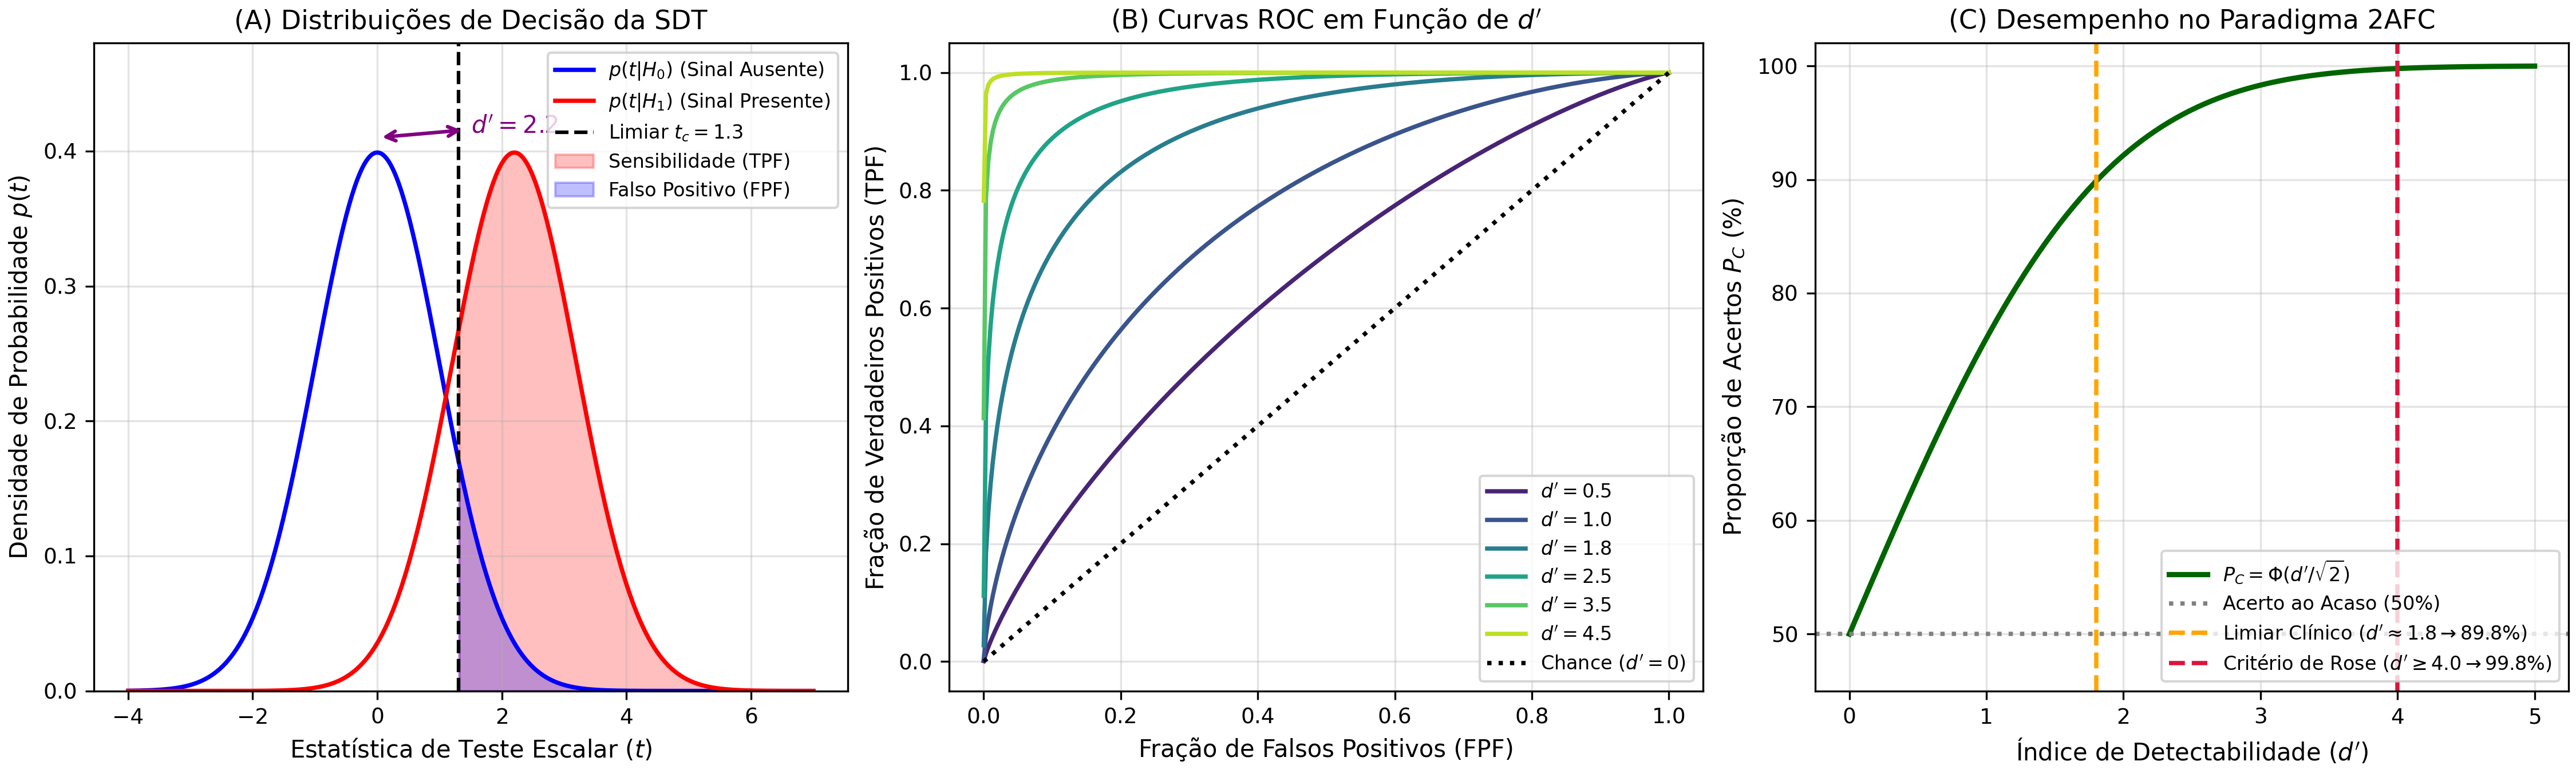
\includegraphics[width=0.98\textwidth]{figuras/fig1_sdt_roc_2afc.png}
  \caption{Fundamentos da Teoria de Detecção de Sinais (SDT), Curvas ROC e Psicofísica 2AFC. (A) Distribuições condicionais de probabilidade $p(t|H_0)$ e $p(t|H_1)$, ilustrando o limiar de decisão $t_c$, a taxa de verdadeiros positivos (TPF) e falsos positivos (FPF), e a separação $d'$. (B) Família de curvas ROC para diferentes índices de detectabilidade ($d' = 0{,}5$ a $4{,}5$). (C) Relação psicofísica formal $P_C = \Phi(d'/\sqrt{2})$ no paradigma 2AFC, destacando o limiar clínico e o critério de Rose.}
  \label{fig:sdt_roc_2afc}
\end{figure}

A variação do limiar $t_c$ permite construir a curva Característica de Operação do Receptor (curva ROC), cujas ordenadas representam a Fração de Verdadeiros Positivos (TPF ou Sensibilidade) e as abscissas indicam a Fração de Falsos Positivos (FPF ou $1 - \text{Especificidade}$) \cite{metz1986}:
\begin{equation}
  \text{TPF}(t_c) = \int_{t_c}^{\infty} p(t|H_1) \, dt, \qquad \text{FPF}(t_c) = \int_{t_c}^{\infty} p(t|H_0) \, dt
  \label{eq:tpf_fpf}
\end{equation}

A integral sob a curva ROC define a métrica global de acurácia, denominada Área sob a Curva ROC (AUC), que varia de $0{,}5$ (desempenho equivalente ao acaso puro) até $1{,}0$ (discriminação perfeita sem erros).

\section{O Índice de Detectabilidade no Domínio Espacial}
\label{sec:dprime_espacial}

Quando as distribuições condicionais $p(t|H_0)$ e $p(t|H_1)$ são gaussianas com variâncias semelhantes, a separação estatística entre elas é sintetizada pelo Índice de Detectabilidade ($d'$):
\begin{equation}
  d' = \frac{\langle t | H_1 \rangle - \langle t | H_0 \rangle}{\sqrt{\frac{1}{2}\sigma^2(t|H_1) + \frac{1}{2}\sigma^2(t|H_0)}}
  \label{eq:dprime_definicao}
\end{equation}

Para a classe dos observadores lineares, a estatística $t$ é obtida pelo produto interno entre a imagem $\mathbf{g}$ e um vetor de template (filtro linear) $\mathbf{w} \in \mathbb{R}^N$:
\begin{equation}
  t = \mathbf{w}^T \mathbf{g} = \sum_{i=1}^N w_i g_i
  \label{eq:template_linear}
\end{equation}

Substituindo essa relação linear na definição de $d'$:
\begin{itemize}
  \item O valor esperado sob $H_0$ é $\langle t | H_0 \rangle = \mathbf{w}^T \langle \mathbf{b} \rangle$;
  \item O valor esperado sob $H_1$ é $\langle t | H_1 \rangle = \mathbf{w}^T \langle \mathbf{b} \rangle + \mathbf{w}^T \mathbf{s}$;
  \item A diferença entre as médias das hipóteses é dada por $\Delta \langle t \rangle = \mathbf{w}^T \mathbf{s}$;
  \item A variância do teste para ruído de matriz de covariância $\mathbf{K} = \langle (\mathbf{b} - \langle \mathbf{b} \rangle)(\mathbf{b} - \langle \mathbf{b} \rangle)^T \rangle$ é $\sigma^2(t) = \mathbf{w}^T \mathbf{K} \mathbf{w}$.
\end{itemize}

Assim, obtém-se a formulação geral do índice de detectabilidade linear no domínio espacial:
\begin{equation}
  d' = \frac{\mathbf{w}^T \mathbf{s}}{\sqrt{\mathbf{w}^T \mathbf{K} \mathbf{w}}}
  \label{eq:dprime_linear_espacial}
\end{equation}

Em termos intuitivos, o numerador ($\mathbf{w}^T \mathbf{s}$) quantifica quanta energia útil do sinal o filtro $\mathbf{w}$ consegue capturar, enquanto o denominador ($\sqrt{\mathbf{w}^T \mathbf{K} \mathbf{w}}$) mede a quantidade de ruído indesejado que atravessa esse mesmo filtro. O valor de $d'$ representa, portanto, a relação sinal-ruído efetiva do observador na tarefa.

\section{Transição para o Domínio das Frequências via Teorema de Wiener-Khinchin}
\label{sec:wiener_khinchin}

A manipulação da matriz de covariância $\mathbf{K}$ no domínio espacial torna-se computacionalmente inviável para imagens de alta resolução (onde $N \approx 262.144$ pixels).

Entretanto, se o ruído de fundo for estacionário no sentido amplo (WSS), a autocorrelação entre dois pontos espaciais depende exclusivamente da distância relativa entre eles. Matematicamente, isso transforma a matriz de covariância em uma matriz circulante.

Pelo Teorema de Wiener-Khinchin, a Transformada de Fourier bidimensional da função de autocorrelação espacial é exatamente igual à densidade espectral de potência do ruído, denominada Espectro de Potência do Ruído ($NPS(u, v)$) \cite{barrett_myers_2004, wagner1979}. Essa propriedade permite transpor o cálculo de $d'$ para integrais contínuas no domínio das frequências espaciais.

A \cref{fig:spectral_metrics} ilustra as quatro grandezas espectrais que compõem o cálculo da detectabilidade.

\begin{figure}[htbp]
  \centering
  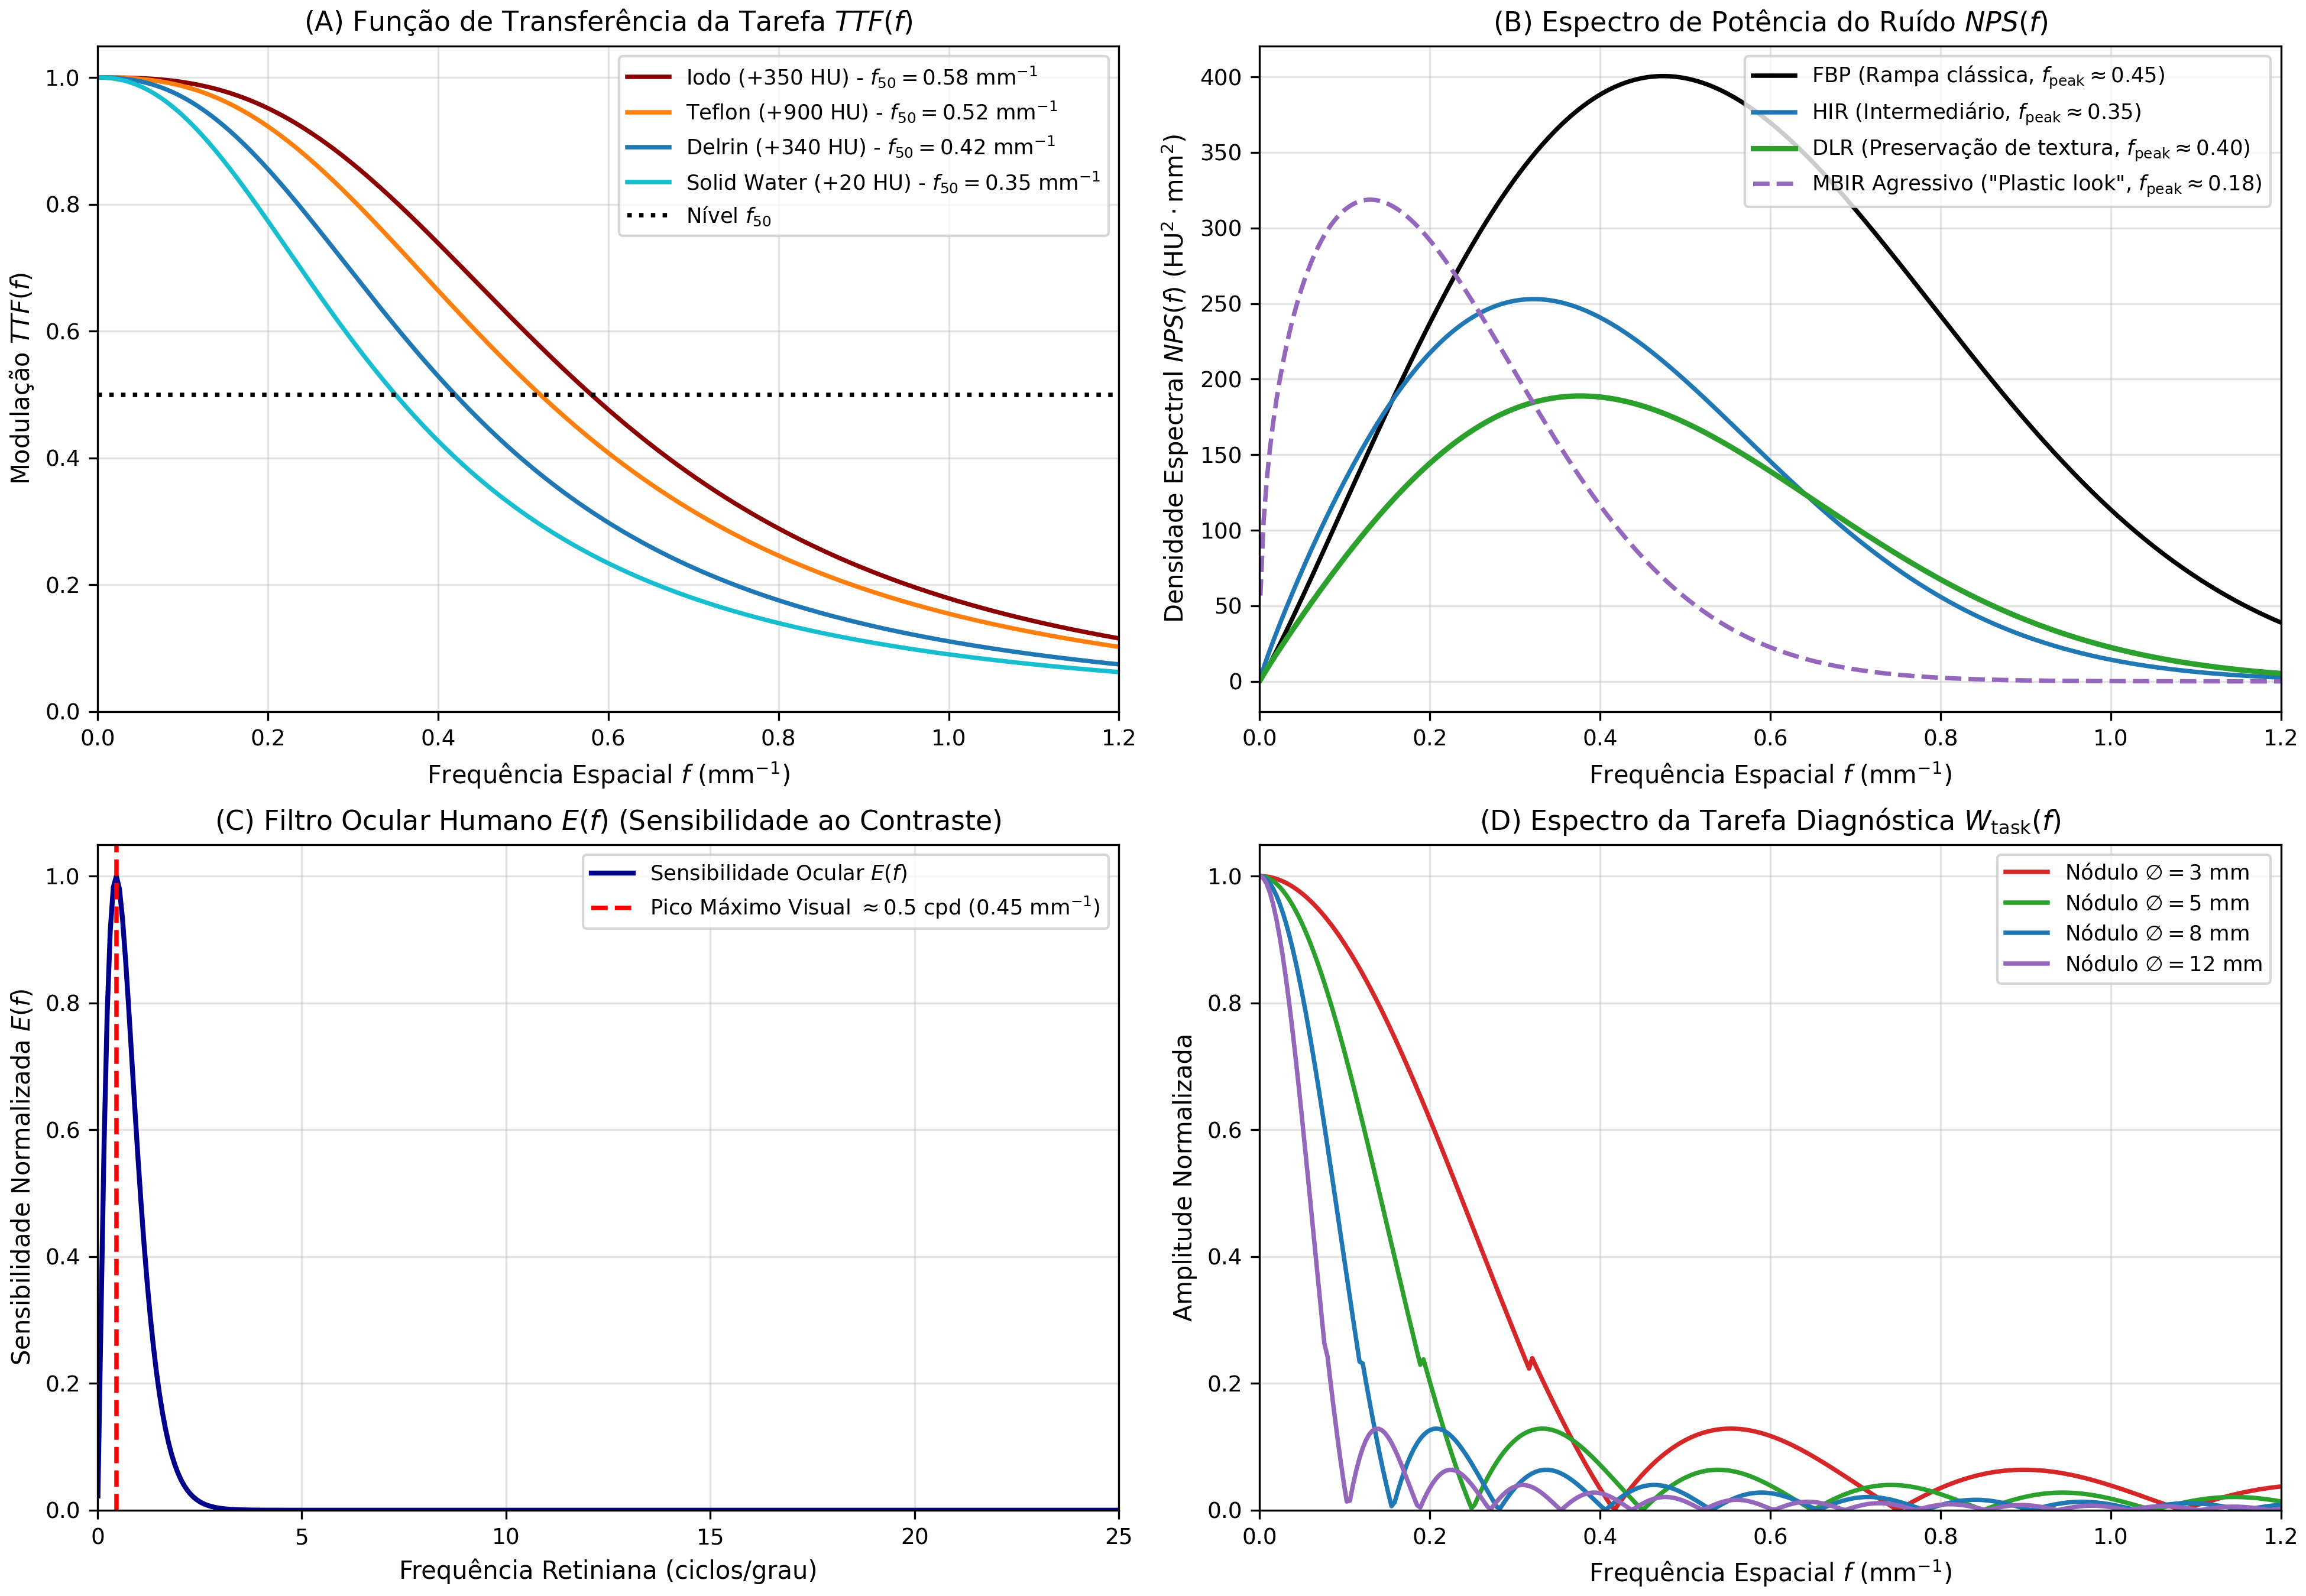
\includegraphics[width=0.98\textwidth]{figuras/fig2_spectral_metrics.png}
  \caption{Métricas Espectrais de Qualidade de Imagem Baseada em Tarefas. (A) Função de Transferência da Tarefa $TTF(f)$ para insertos de diferentes contrastes e materiais, evidenciando a dependência não linear e o ponto de modulação de 50\% ($f_{50}$). (B) Espectro de Potência do Ruído $NPS(f)$ comparando FBP (rampa de alta frequência), HIR, DLR e MBIR com deslocamento de $f_{\text{peak}}$ (``plastic look''). (C) Filtro Ocular Humano $E(f)$ (Função de Sensibilidade ao Contraste). (D) Espectro de Potência da Tarefa Diagnóstica $W_{\text{task}}(f)$ para lesões nodulares esféricas de diferentes diâmetros ($\varnothing = 3, 5, 8, 12\text{ mm}$).}
  \label{fig:spectral_metrics}
\end{figure}

\subsection{Função de Transferência da Tarefa e Resolução Dependente de Contraste}
A Função de Transferência da Tarefa ($TTF(f)$) quantifica a resolução espacial do tomógrafo para um contraste radiológico e nível de dose específicos \cite{aapm_tg233_2019}. Ela é obtida experimentalmente através da técnica da borda circular em insertos cilíndricos de calibração (Painel A da \cref{fig:spectral_metrics}).

O cálculo segue três etapas analíticas:
\begin{enumerate}
  \item Obtenção do perfil radial de atenuação em torno do centro geométrico do inserto, gerando a Função de Resposta ao Degrau Radial ($\text{ESF}(r)$);
  \item Diferenciação numérica radial para obter a Função de Espalhamento de Linha:
  \begin{equation}
    \text{LSF}(r) = \frac{d}{dr}\text{ESF}(r)
    \label{eq:lsf}
  \end{equation}
  \item Cálculo da Transformada de Fourier 1D normalizada na frequência zero:
  \begin{equation}
    TTF(f) = \frac{\left| \int_{-\infty}^{\infty} \text{LSF}(r) e^{-i 2\pi f r} \, dr \right|}{\left| \int_{-\infty}^{\infty} \text{LSF}(r) \, dr \right|}
    \label{eq:ttf_formula}
  \end{equation}
\end{enumerate}

A frequência $f_{50}$ representa o ponto no qual a transferência de contraste decai para 50\% do valor máximo, servindo como índice de nitidez do protocolo.

\subsection{Espectro de Potência do Ruído e Textura Espacial}
O Espectro de Potência do Ruído 2D ($NPS(u, v)$) quantifica como a energia do ruído estocástico se distribui pelas frequências espaciais da imagem:
\begin{equation}
  NPS(u, v) = \frac{\Delta x \Delta y}{N_x N_y} \left\langle \left| \mathcal{F}_{2D} \left\{ I(x, y) - \overline{I}(x, y) \right\} \right|^2 \right\rangle
  \label{eq:nps_formula}
\end{equation}
onde $\overline{I}(x, y)$ é a superfície de fundo removida por \emph{detrending}.

Para caracterizar a textura visual do ruído, calcula-se a frequência de pico ($f_{\text{peak}}$) e a frequência média ponderada ($f_{\text{av}}$):
\begin{equation}
  f_{\text{av}} = \frac{\int_{0}^{\infty} f \cdot NPS(f) \, df}{\int_{0}^{\infty} NPS(f) \, df}
  \label{eq:fav}
\end{equation}

Conforme demonstrado no Painel B da \cref{fig:spectral_metrics}, algoritmos analíticos (FBP) apresentam picos em frequências mais elevadas (textura granular fina), enquanto métodos iterativos agressivos deslocam o pico para frequências baixas, provocando perda de textura estocástica natural (\emph{plastic look}).

\subsection{Filtro Ocular e Modelagem Biofísica da Visão Humana}
O olho humano não responde de forma uniforme a todas as frequências espaciais. A Função de Sensibilidade ao Contraste do sistema visual atua como um filtro passa-faixa, modelado matematicamente pelo Filtro Ocular $E(f)$ \cite{burgess1994, aapm_tg233_2019}:
\begin{equation}
  E(f) = \left( \frac{f}{f_0} \right)^n \exp\left[ -c \left( \frac{f}{f_0} \right)^m \right]
  \label{eq:eye_filter}
\end{equation}
com parâmetros $f_0 = 0{,}8 \text{ cpd}$, $n = 1{,}3$, $m = 1{,}1$ e $c = 2{,}2$.

A frequência angular na retina ($f_{\text{retina}}$, em ciclos por grau) relaciona-se com a frequência espacial física na imagem ($f_{\text{imagem}}$, em $\text{mm}^{-1}$) para uma distância de visualização de $500 \text{ mm}$ através da expressão:
\begin{equation}
  f_{\text{retina}} (\text{ciclos/grau}) \approx 8{,}727 \cdot f_{\text{imagem}} (\text{mm}^{-1})
  \label{eq:fretina}
\end{equation}

O Painel C da \cref{fig:spectral_metrics} evidencia que o olho humano possui máxima sensibilidade a variações de contraste na faixa de 3 a 5 ciclos/grau ($\approx 0{,}45 \text{ mm}^{-1}$ no plano do monitor diagnóstico), atenuando tanto variações muito suaves quanto detalhes ultrafinos.

Adicionalmente, a fisiologia da visão introduz um ruído interno neural ($\sigma_{\text{int}}^2$), de modo que a detectabilidade humana real relaciona-se com o modelo computacional por:
\begin{equation}
  d'_{\text{humano}} = \frac{d'_{\text{NPWE}}}{\sqrt{1 + \left(\frac{\sigma_{\text{int}}}{\sigma_{\text{ext}}}\right)^2}}
  \label{eq:dprime_humano_int}
\end{equation}

\subsection{Espectro da Tarefa Diagnóstica e o Critério de Rose}
Para uma lesão circular homogênea de raio $R$ e contraste central $\Delta C$, o espectro da tarefa diagnóstica no domínio de Fourier é descrito por uma função de Bessel ordinária de primeira espécie $J_1$:
\begin{equation}
  W_{\text{task}}(f) = \Delta C \cdot 2\pi R^2 \left| \frac{J_1(2\pi R f)}{2\pi R f} \right|
  \label{eq:wtask}
\end{equation}

O Painel D da \cref{fig:spectral_metrics} mostra que lesões maiores concentram sua energia em frequências espaciais baixas, enquanto lesões puntiformes dispersam sua informação em frequências médias e altas.

O Critério clássico de Rose \cite{rose1948} postulava que um sinal só é detectado pelo ser humano se a relação de contraste-ruído ponderada pela área for superior a 5 ($k \ge 5$). Na formulação contemporânea da TBIQ, esse limiar corresponde a $d' \ge 4{,}0 \text{ a } 5{,}0$ para detecção quase certa ($P_C \ge 99\%$), enquanto $d' \approx 1{,}5 \text{ a } 2{,}0$ estabelece o limite de visibilidade clínica aceitável.

\section{Paradigmas de Detecção e a Dedução Matemática do Experimento 2AFC}
\label{sec:2afc_deducao}

O padrão-ouro experimental para medir a percepção humana em física médica é o experimento de Escolha Forçada entre Duas Alternativas (2AFC) \cite{burgess2011, eckstein2000}.

No teste 2AFC, apresentam-se ao leitor dois campos de imagem idênticos: um contendo apenas ruído ($H_0$) e outro contendo a lesão inserida sobre o ruído ($H_1$). O observador avalia as duas imagens e calcula suas respectivas variáveis de decisão: $t_0 = t(\mathbf{g}|H_0)$ e $t_1 = t(\mathbf{g}|H_1)$. O observador acerta a escolha se $t_1 > t_0$.

Considerando que $t_0 \sim \mathcal{N}(\mu_0, \sigma^2)$ e $t_1 \sim \mathcal{N}(\mu_1, \sigma^2)$ são variáveis normais independentes, definimos a variável de diferença $\Delta t = t_1 - t_0$.

As propriedades estatísticas dessa variável combinada são:
\begin{itemize}
  \item Média da diferença: $\mu_{\Delta t} = \mu_1 - \mu_0$;
  \item Variância da diferença: $\sigma_{\Delta t}^2 = \sigma^2(t_1) + \sigma^2(t_0) = 2\sigma^2$;
  \item Desvio padrão da diferença: $\sigma_{\Delta t} = \sqrt{2}\sigma$.
\end{itemize}

A proporção de acertos esperada ($P_C$) é a probabilidade de que $\Delta t > 0$:
\begin{equation}
  P_C = P(\Delta t > 0) = P\left( \frac{\Delta t - \mu_{\Delta t}}{\sigma_{\Delta t}} > \frac{-(\mu_1 - \mu_0)}{\sqrt{2}\sigma} \right) = \Phi\left( \frac{\mu_1 - \mu_0}{\sqrt{2}\sigma} \right)
  \label{eq:pc_2afc_step}
\end{equation}

Como $d' = \frac{\mu_1 - \mu_0}{\sigma}$, estabelece-se a relação fundamental da psicofísica 2AFC:
\begin{equation}
  P_C = \Phi\left( \frac{d'}{\sqrt{2}} \right)
  \label{eq:pc_dprime_2afc}
\end{equation}

Invertendo a equação através da função cumulativa normal inversa $\Phi^{-1}$:
\begin{equation}
  d'_{\text{humano}} = \sqrt{2} \cdot \Phi^{-1}(P_C)
  \label{eq:dprime_humano_inversa}
\end{equation}

Essa dedução demonstra a origem física do fator $\sqrt{2}$, permitindo converter a porcentagem de acertos de médicos radiologistas em um índice escalar de detectabilidade $d'$ diretamente comparável aos modelos matemáticos.

\chapter{A Evolução dos Observadores de Modelo Lineares e Validação Psicofísica MRMC}
\label{chap:observadores_lineares}

\section{O Observador Ideal Bayesiano e o Limite Superior Termodinâmico}
\label{sec:io}

O Observador Ideal (IO) representa o tomador de decisão estatístico ótimo que utiliza todas as informações físicas do feixe de radiação e do detector para maximizar a área sob a curva ROC ($AUC$), de acordo com o Lema de Neyman-Pearson \cite{barrett_myers_2004}.

A estatística de teste do Observador Ideal para ruído gaussiano com matriz de covariância $\mathbf{K}$ e sinal determinístico $\mathbf{s}$ é obtida pelo logaritmo da razão de verossimilhança:
\begin{equation}
  t_{\text{IO}}(\mathbf{g}) = \mathbf{s}^T \mathbf{K}^{-1} \mathbf{g}
  \label{eq:io_estatistica}
\end{equation}

O índice de detectabilidade do Observador Ideal é expresso pela distância de Mahalanobis:
\begin{equation}
  d'_{\text{IO}} = \sqrt{\mathbf{s}^T \mathbf{K}^{-1} \mathbf{s}} = \left[ \iint \frac{\left| W_{\text{task}}(u, v) \cdot TTF(u, v) \right|^2}{NPS(u, v)} \, du \, dv \right]^{1/2}
  \label{eq:io_dprime}
\end{equation}

O Observador Ideal executa uma operação de pré-branqueamento (\emph{prewhitening} $\mathbf{K}^{-1/2}$), descorrelacionando completamente a estrutura de ruído antes de aplicar o filtro casado. Embora o IO estabeleça o limite físico máximo de informação contida na radiação, ele superestima grosseiramente a percepção de observadores humanos, servindo apenas como referência física teórica superior.

\section{O Observador NPW e a Dedução Contínua do Modelo NPWE}
\label{sec:npwe}

Para aproximar os modelos matemáticos das limitações biológicas, desenvolveu-se o modelo sem pré-branqueamento (\emph{Non-Prewhitening} --- NPW), cuja premissa é que o olho humano não inverte matrizes de ruído, atuando como um filtro casado simples $\mathbf{w}_{\text{NPW}} = \mathbf{s}$ \cite{burgess1994}.

A incorporação do filtro ocular $E(f)$ deu origem ao modelo NPWE (\emph{Non-Prewhitening with Eye Filter}), que foi adotado pelo relatório internacional AAPM TG-233 como referência normativa para a avaliação de tomógrafos clínicos \cite{aapm_tg233_2019}.

Aplicando a diagonalização do Teorema de Wiener-Khinchin, a detectabilidade do modelo NPWE em coordenadas contínuas bidimensionais é descrita por:
\begin{equation}
  d'_{\text{NPWE}} = \frac{\iint \left| W_{\text{task}}(u, v) \right|^2 \cdot \left[ TTF(u, v) \right]^2 \cdot \left[ E(u, v) \right]^2 \, du \, dv}{\left\{ \iint \left| W_{\text{task}}(u, v) \right|^2 \cdot \left[ TTF(u, v) \right]^2 \cdot \left[ E(u, v) \right]^4 \cdot NPS(u, v) \, du \, dv \right\}^{1/2}}
  \label{eq:dprime_npwe_2d}
\end{equation}

Para sistemas com simetria rotacional no plano de corte axial, a integral é simplificada para a coordenada radial $f$:
\begin{equation}
  d'_{\text{NPWE}} = \frac{\int_{0}^{\infty} \left| W_{\text{task}}(f) \right|^2 \cdot \left[ TTF(f) \right]^2 \cdot \left[ E(f) \right]^2 \cdot 2\pi f \, df}{\left\{ \int_{0}^{\infty} \left| W_{\text{task}}(f) \right|^2 \cdot \left[ TTF(f) \right]^2 \cdot \left[ E(f) \right]^4 \cdot NPS(f) \cdot 2\pi f \, df \right\}^{1/2}}
  \label{eq:dprime_npwe_radial}
\end{equation}

O modelo NPWE apresenta excelente correlação com leitores humanos em fundos homogêneos. No entanto, ele falha sistematicamente quando aplicado a fundos anatômicos complexos, pois não possui mecanismos para tratar o ruído estrutural.

\section{O Desafio dos Fundos Estruturados: Hotelling Observer e Channelized Hotelling Observer}
\label{sec:cho}

\subsection{Formulação Algébrica do Observador de Hotelling}
Quando uma lesão está localizada sobre tecidos anatômicos reais (como o parênquima pulmonar ou o trabeculado ósseo), o fundo introduz uma componente adicional de ruído estrutural. A matriz de covariância total é dada por $\mathbf{K}_{\text{total}} = \mathbf{K}_{\text{ruído}} + \mathbf{K}_{\text{anatômico}}$ \cite{barrett_myers_2004}.

O Observador de Hotelling (HO) aplica a análise discriminante linear de Fisher para maximizar a separabilidade de classes sob fundos variáveis:
\begin{equation}
  \mathbf{w}_{\text{HO}} = \mathbf{K}_{\text{total}}^{-1} \langle \mathbf{s} \rangle \implies d'_{\text{HO}} = \sqrt{\langle \mathbf{s} \rangle^T \mathbf{K}_{\text{total}}^{-1} \langle \mathbf{s} \rangle}
  \label{eq:ho_formulation}
\end{equation}

\subsection{Modelagem dos Canais Corticais: Gabor, Laguerre-Gauss e D-DOG}
Para simular o processamento de imagens realizado pelos neurônios do córtex visual primário (área V1) e contornar o custo computacional da inversão da matriz $\mathbf{K}_{\text{total}}$, Barrett et al. \cite{barrett1993}, Yao \& Barrett \cite{yao1992} e Myers \& Barrett \cite{myers1987} introduziram o Observador de Hotelling Canalizado (\emph{Channelized Hotelling Observer} --- CHO).

O CHO aplica uma matriz de canais corticais $\mathbf{T} \in \mathbb{R}^{C \times N}$ (onde $C \ll N$, tipicamente $C \in [4, 10]$ canais), reduzindo o vetor de imagem $\mathbf{g}$ a um vetor canalizado de baixa dimensionalidade $\mathbf{v} \in \mathbb{R}^C$:
\begin{equation}
  \mathbf{v} = \mathbf{T} \mathbf{g}
  \label{eq:cho_reduction}
\end{equation}

O fluxo completo de processamento do modelo CHO está ilustrado no \cref{fig:cho_flow}.

\begin{figure}[htbp]
  \centering
  
\includegraphics[width=0.95\textwidth]{figuras/flow3_cho_pipeline.png}
  \caption{Decomposição Cortical e Processamento de Decisão no Channelized Hotelling Observer (CHO).}
  \label{fig:cho_flow}
\end{figure}

A matriz de covariância no espaço dos canais $\mathbf{K}_{\mathbf{v}} = \mathbf{T} \mathbf{K}_{\text{total}} \mathbf{T}^T \in \mathbb{R}^{C \times C}$ é facilmente invertida, fornecendo o índice de detectabilidade do CHO:
\begin{equation}
  d'_{\text{CHO}} = \sqrt{\langle \mathbf{v}_{\mathbf{s}} \rangle^T \mathbf{K}_{\mathbf{v}}^{-1} \langle \mathbf{v}_{\mathbf{s}} \rangle}
  \label{eq:dprime_cho}
\end{equation}

A \cref{fig:cho_channels} apresenta os três principais modelos de canais corticais utilizados na literatura.

\begin{figure}[htbp]
  \centering
  
\includegraphics[width=0.98\textwidth]{figuras/fig3_cho_cortical_channels.png}
  \caption{Modelagem de Canais Corticais no Channelized Hotelling Observer (CHO). (A) Resposta em frequência dos canais passa-faixa Dense Difference of Gaussians (D-DOG) com espaçamento de meia oitava. (B) Perfis espaciais dos canais Laguerre-Gauss radiais ($LG_0$ a $LG_3$). (C) Mapa de sensibilidade bidimensional de um canal de Gabor orientado a $\theta = 45^\circ$. (D) Comportamento da detectabilidade $d'$ do modelo CHO em ruído anatômico estruturado comparado ao colapso do modelo NPWE não-canalizado.}
  \label{fig:cho_channels}
\end{figure}

As formulações matemáticas dos canais corticais são:
\begin{enumerate}
  \item \textbf{Canais D-DOG (\emph{Dense Difference of Gaussians}):} Filtros passa-faixa concêntricos com espaçamento de meia oitava ($\alpha = 1{,}4$) e razão $a = 1{,}6$:
  \begin{equation}
    D\text{-}DOG_j(f) = \exp\left[ -\frac{f^2}{2\sigma_j^2} \right] - \exp\left[ -\frac{f^2}{2(a \sigma_j)^2} \right]
    \label{eq:ddog}
  \end{equation}
  \item \textbf{Canais Laguerre-Gauss (LG):} Funções ortogonais com simetria circular ponderadas por Polinômios de Laguerre $L_n$:
  \begin{equation}
    LG_n(r; a_u) = \frac{\sqrt{2}}{a_u} \exp\left( -\frac{\pi r^2}{a_u^2} \right) L_n\left( \frac{2\pi r^2}{a_u^2} \right)
    \label{eq:lg}
  \end{equation}
  \item \textbf{Canais de Gabor:} Funções sinusoidais moduladas por envelope gaussiano com orientação espacial $\theta$ e frequência foveal $f_c$ \cite{abbey2001}.
\end{enumerate}

\section{Validação Psicofísica e Decomposição Formal da Variância na ANOVA MRMC}
\label{sec:mrmc}

\subsection{Modelo Linear Misto de Efeitos Aleatórios}
Para certificar a confiabilidade metrológica de um observador computacional, é imperativo comparar seus resultados com o desempenho de médicos radiologistas reais em estudos psicofísicos 2AFC sob análise estatística \emph{Multi-Reader Multi-Case} (MRMC) \cite{dorfman1992, obuchowski1995, hillis2011, racine2021}.

O paradigma MRMC isola a variabilidade inerente aos leitores humanos da variabilidade amostral dos pacientes (casos clínicos). O modelo linear misto de Dorfman-Berbaum-Metz (DBM) e Obuchowski-Rockette-Hillis (ORH) decompõe a acurácia observada $Y_{ijk}$ (para a modalidade $i$, leitor $j$ e caso $k$) em:
\begin{equation}
  Y_{ijk} = \mu + \tau_i + R_j + C_k + (\tau R)_{ij} + (\tau C)_{ik} + (RC)_{jk} + \epsilon_{ijk}
  \label{eq:mrmc_anova}
\end{equation}
onde:
\begin{itemize}
  \item $\mu$ é a média global de acurácia;
  \item $\tau_i$ é o efeito fixo da modalidade tomográfica $i$;
  \item $R_j \sim \mathcal{N}(0, \sigma^2_R)$ é o efeito aleatório do leitor $j$;
  \item $C_k \sim \mathcal{N}(0, \sigma^2_C)$ é o efeito aleatório do caso clínico $k$;
  \item $(\tau R)_{ij} \sim \mathcal{N}(0, \sigma^2_{\tau R})$ é a interação modalidade $\times$ leitor;
  \item $(\tau C)_{ik} \sim \mathcal{N}(0, \sigma^2_{\tau C})$ é a interação modalidade $\times$ caso;
  \item $(RC)_{jk} \sim \mathcal{N}(0, \sigma^2_{RC})$ é a interação leitor $\times$ caso;
  \item $\epsilon_{ijk} \sim \mathcal{N}(0, \sigma^2_{\epsilon})$ é o erro residual aleatório.
\end{itemize}

\subsection{Graus de Liberdade Ajustados de Satterthwaite e Teste de Hipóteses}
A estatística de teste $F$ para a hipótese de equivalência entre o modelo computacional e os leitores humanos ($H_0: \tau_{\text{modelo}} = \tau_{\text{humano}}$) utiliza a aproximação de Satterthwaite para os graus de liberdade efetivos do denominador ($df_{\text{den}}$):
\begin{equation}
  F = \frac{MS(\tau)}{MS(\tau R) + MS(\tau C) - MS(\tau RC)} \sim F(df_{\text{num}}, df_{\text{den}})
  \label{eq:satterthwaite}
\end{equation}

Exige-se que o Coeficiente de Correlação Intraclasse ($ICC$) atinja $ICC \ge 0{,}90$ com intervalo de confiança de 95\% para que o modelo computacional seja aceito como substituto metrológico confiável da avaliação humana.

\chapter{O Colapso da Linearidade, Algoritmos DLR e Simuladores Híbridos}
\label{chap:colapso_linearidade}

\section{Taxonomia e Comparativo Físico dos Algoritmos de Reconstrução}
\label{sec:taxonomia_dlr}

A evolução algorítmica da tomografia computadorizada compreende quatro gerações principais de processamento numérico de sinogramas.

A \cref{tab:taxonomia_algoritmos} detalha os algoritmos comerciais implementados pelos quatro principais fabricantes globais de tomógrafos.

\begin{table}[htbp]
  \centering
  \small
  \caption{Taxonomia dos algoritmos comerciais de reconstrução tomográfica por fabricante.}
  \label{tab:taxonomia_algoritmos}
  \begin{tabularx}{\textwidth}{lXXX}
    \toprule
    \textbf{Fabricante} & \textbf{Reconstrução Iterativa Híbrida (HIR)} & \textbf{Reconstrução Iterativa Baseada em Modelos (MBIR)} & \textbf{Reconstrução por Aprendizado Profundo (DLR)} \\
    \midrule
    \textbf{GE Healthcare} & ASiR / ASiR-V & Veo & \textbf{TrueFidelity} (treinado com FBP de dose plena) \\
    \textbf{Canon Medical} & AIDR 3D / AIDR 3D Enhanced & FIRST & \textbf{AiCE} (\emph{Advanced intelligent Clear-IQ Engine}) \\
    \textbf{Siemens Healthineers} & SAFIRE / ADMIRE & REDUCE & \textbf{Precise Image} / \textbf{Alpha Engine} (PCCT) \\
    \textbf{Philips Healthcare} & iDose4 & IMR (\emph{Iterative Model Reconstruction}) & \textbf{Precise Image} (redes convolucionais profundas) \\
    \bottomrule
  \end{tabularx}
\end{table}

\subsection{Filosofia GE Healthcare: TrueFidelity e Mapeamento Direto de FBP}
A rede neural profunda do TrueFidelity (GE Healthcare) foi concebida sob uma filosofia de preservação textural estrita. Seu treinamento supervisionado utilizou como alvo (\emph{ground truth}) imagens reconstruídas por FBP adquiridas em dose plena (alta contagem de fótons). Dessa forma, a rede aprende a remover o ruído quântico de exames de baixa dose sem alterar o formato de rampa do $NPS(f)$, preservando a granularidade visual clássica apreciada por radiologistas experientes.

\subsection{Filosofia Canon Medical: AiCE e Treinamento Ancorado em MBIR}
O algoritmo AiCE (\emph{Advanced intelligent Clear-IQ Engine}, Canon Medical) adota como alvo de treinamento imagens reconstruídas por MBIR de altíssima qualidade (algoritmo FIRST). Como o MBIR modela a óptica real do feixe e a física do ponto focal, a rede aprende a recuperar frequências espaciais elevadas em bordas ($TTF$ elevada) e atua com forte supressão de ruído em tecidos moles, exigindo calibração criteriosa para evitar a suavização excessiva de microestruturas.

\subsection{Filosofia Siemens Healthineers: Precise Image e Alpha Engine}
A Siemens Healthineers desenvolveu redes neurais que atuam de forma combinada no domínio de projeções brutas e no espaço da imagem. Em sistemas PCCT, o algoritmo \emph{Alpha Engine} processa múltiplos sinogramas espectrais simultaneamente, aplicando regularização adaptativa de gradientes que mantém a resolução espacial mesmo em níveis ultrabaixos de dose ($\text{CTDI}_{\text{vol}} < 1{,}0\text{ mGy}$).

\subsection{Filosofia Philips Healthcare: Precise Image em Espaço Híbrido}
O sistema Precise Image da Philips utiliza redes convolucionais profundas em múltiplas escalas com camadas residuais, processando dados iterativamente entre o espaço de sinogramas e o domínio espacial para eliminar artefatos de feixe endurecido e espalhamento com baixo custo computacional.

\section{A Quebra da Linearidade, Não-Estacionariedade e o Efeito Ceroso}
\label{sec:quebra_linearidade}

Em sistemas tomográficos que utilizam reconstruções por aprendizado profundo (DLR) e MBIR, a relação matemática entre as projeções brutas $\mathbf{y}$ e a imagem final $\mathbf{x}$ é estritamente não linear \cite{greffier2026, debbiche2024}:
\begin{equation}
  \mathbf{x} = \mathcal{R}_{\text{DLR}}(\mathbf{y}) \ne \mathbf{A}^\dagger \mathbf{y}
  \label{eq:nao_linear_dlr}
\end{equation}

Essa não-linearidade acarreta fenômenos físicos complexos, evidenciados na \cref{fig:dlr_non_linear}:
\begin{enumerate}
  \item \textbf{Dependência do Contraste e da Cena:} A resolução espacial da imagem deixa de ser constante, variando dinamicamente de acordo com o contraste do objeto e o nível de ruído local;
  \item \textbf{Não-Estacionariedade Espacial:} O ruído da imagem não possui propriedades estatísticas homogêneas. Em torno de bordas de alto contraste, o algoritmo preserva frequências espaciais elevadas, enquanto em regiões homogêneas de tecidos moles atua com agressiva remoção de ruído;
  \item \textbf{Efeito Ceroso (\emph{Plastic/Waxy Look}):} A excessiva concentração de energia do ruído em frequências baixas gera uma textura artificialmente lisa, que mascara lesões sutis de baixo contraste e reduz a sensibilidade de radiologistas \cite{toia2023, greffier2026};
  \item \textbf{Colapso dos Modelos Lineares Tradicionais:} O modelo analítico linear NPWE falha em prever a acurácia diagnóstica real sob reconstruções DLR, apresentando dispersão acentuada e baixa correlação ($r \approx 0{,}68$, Painel B da \cref{fig:dlr_non_linear}).
\end{enumerate}

\begin{figure}[htbp]
  \centering
  
\includegraphics[width=0.98\textwidth]{figuras/fig4_dlr_non_linearity_detrending.png}
  \caption{Impacto da Não-Linearidade em DLR, Colapso de Modelos Analíticos Lineares e Metodologia de Detrending. (A) Detectabilidade $d'$ em função do nível de dose $\text{CTDI}_{\text{vol}}$ para FBP, HIR e DLR. (B) Dispersão e quebra de correlação linear do modelo NPWE ($r = 0{,}68$) versus a alta correlação do modelo DLMO ancorado na percepção de radiologistas ($r = 0{,}98$). (C) Processo de Detrending Polinomial 2D: remoção do gradiente anatômico macroscópico $P_2(x, y)$ para isolamento do ruído quântico puro $\delta I(x, y)$.}
  \label{fig:dlr_non_linear}
\end{figure}

\section{A Transição dos Simuladores: De Cilindros Homogêneos a Phantoms Antropomórficos Híbridos}
\label{sec:phantoms_hibridos}

Simuladores físicos homogêneos de acrílico ou água (como o \emph{phantom} Catphan\textregistered) foram desenvolvidos para a calibração de sistemas FBP lineares. Quando submetidos a algoritmos DLR (que foram treinados predominantemente com anatomias humanas reais), esses simuladores produzem padrões atípicos fora da distribuição de treinamento, invalidando as medições metrológicas \cite{solomon2020, racine2020}.

Para restabelecer o rigor da avaliação física, a física médica adotou a metodologia dos \emph{Phantoms} Antropomórficos Híbridos (\cref{fig:phantom_flow}).

\begin{figure}[htbp]
  \centering
  
\includegraphics[width=0.95\textwidth]{figuras/flow4_phantom_hibrido_2afc.png}
  \caption{Metodologia Experimental com Phantoms Físicos Antropomórficos, Inserção Híbrida de Lesões 3D e Plataforma Psicofísica 2AFC.}
  \label{fig:phantom_flow}
\end{figure}

Essa abordagem utiliza simuladores físicos de alta fidelidade tecidual (como o \emph{phantom} FREDDIE) confeccionados por impressão 3D multimaterial para aquisição de fundos anatômicos reais ($H_0$), sobre os quais são inseridos computacionalmente modelos tridimensionais de lesões convolvidas com a PSF tridimensional do tomógrafo ($H_1$). Isso possibilita a geração de milhares de imagens com verdade de campo exata para treinamento de redes e testes psicofísicos humanos.

\section{Tratamento de Ruído em Anatomias Complexas: Detrending Polinomial 2D e Incerteza Bootstrap}
\label{sec:detrending}

Para calcular o espectro de ruído ($NPS$) no parênquima pulmonar ou no abdome de um \emph{phantom} antropomórfico, é necessário remover as variações anatômicas macroscópicas de densidade através da técnica de \emph{Detrending} Polinomial 2D (Painel C da \cref{fig:dlr_non_linear}):

Para cada sub-região de interesse $I_k(x, y)$, ajusta-se uma superfície polinomial bidimensional de 2ª ordem $P_2(x, y)$ por mínimos quadrados:
\begin{equation}
  P_2(x, y) = a_0 + a_1 x + a_2 y + a_3 x^2 + a_4 y^2 + a_5 xy
  \label{eq:polinomio_2d}
\end{equation}

A matriz de ruído puro residual $\delta I_k(x, y) = I_k(x, y) - P_2(x, y)$ é então submetida a janelamento de Hanning 2D para cálculo do $NPS$ sem vazamento espectral.

Para estimar o erro padrão e os intervalos de confiança de 95\% do índice $d'$ sem impor premissas gaussianas arbitrárias, aplica-se a técnica estatística de reamostragem Bootstrap não-paramétrica com $B = 2000$ replicações com reposição.

\chapter{O Estado da Arte: Observadores por Aprendizado Profundo, PCCT e Otimização Multiobjetivo}
\label{chap:estado_da_arte}

\section{Observadores Baseados em Aprendizado Profundo e Auto-Atenção}
\label{sec:dlmo}

Para superar a quebra de linearidade dos algoritmos DLR, a física médica desenvolveu os Observadores de Modelo Baseados em Aprendizado Profundo (\emph{Deep Learning Model Observers} --- DLMO) \cite{zhou2021, schilder2026}.

Em vez de assumir templates lineares fixos, o DLMO emprega redes neurais profundas com arquitetura \emph{Vision Transformer} (ViT) dotadas de mecanismos de Auto-Atenção Multi-Cabeça (MHSA), conforme esquematizado no \cref{fig:dlmo_arch}.

\begin{figure}[htbp]
  \centering
  
\includegraphics[width=0.95\textwidth]{figuras/flow5_dlmo_architecture.png}
  \caption{Arquitetura Neural do Observador por Aprendizado Profundo (DLMO) com Auto-Atenção Multi-Cabeça (Vision Transformer) e Calibração Perceptual.}
  \label{fig:dlmo_arch}
\end{figure}

\subsection{Arquitetura Vision Transformer: Projeção Linear e Patch Embeddings}
A imagem tomográfica $\mathbf{x} \in \mathbb{R}^{H \times W \times C}$ é dividida em uma sequência de $N_p = \frac{HW}{P^2}$ blocos bidimensionais não-sobrepostos (\emph{patches}) $\mathbf{x}_p \in \mathbb{R}^{N_p \times (P^2 C)}$, onde $P \times P$ é a dimensão espacial de cada bloco \cite{dosovitskiy2021}. Cada bloco é projetado linearmente para um espaço latente de dimensão $D_{\text{model}}$ através de uma matriz treinável $\mathbf{E}$:
\begin{equation}
  \mathbf{z}_0 = \left[ \mathbf{x}_{\text{class}}; \, \mathbf{x}_p^1 \mathbf{E}; \, \mathbf{x}_p^2 \mathbf{E}; \, \dots; \, \mathbf{x}_p^{N_p} \mathbf{E} \right] + \mathbf{E}_{\text{pos}}
  \label{eq:vit_embedding}
\end{equation}
onde $\mathbf{x}_{\text{class}}$ é o token especial de decisão e $\mathbf{E}_{\text{pos}} \in \mathbb{R}^{(N_p + 1) \times D_{\text{model}}}$ codifica as coordenadas espaciais 2D absolutas.

\subsection{Mecanismo de Auto-Atenção Multi-Cabeça e Conexão Neurofisiológica}
A auto-atenção permite à rede computacional aprender correlações espaciais globais e locais simultaneamente. Para cada bloco, calculam-se as projeções de Consulta ($Q$), Chave ($K$) e Valor ($V$):
\begin{equation}
  Q = \mathbf{z} \mathbf{W}_Q, \qquad K = \mathbf{z} \mathbf{W}_K, \qquad V = \mathbf{z} \mathbf{W}_V
  \label{eq:qkv}
\end{equation}

A equação de auto-atenção escalonada por produto escalar é expressa por:
\begin{equation}
  \text{Attention}(Q, K, V) = \text{softmax}\left( \frac{Q K^T}{\sqrt{d_k}} \right) V
  \label{eq:attention_formula}
\end{equation}
onde o fator $\sqrt{d_k}$ evita a saturação dos gradientes na função softmax.

Do ponto de vista neurofisiológico, essa formulação matemática mimetiza a interação foveal-periférica dos radiologistas: a matriz de atenção pondera áreas anatômicas distantes para inferir o contexto anatômico de fundo enquanto focaliza recursos computacionais na detecção foveal da lesão central.

A estatística de teste não linear $t_{\text{DL}}(\mathbf{g}) = f_{\boldsymbol{\theta}}(\mathbf{g})$ permite calcular o índice de detectabilidade não linear:
\begin{equation}
  d'_{\text{DL}} = \frac{\langle f_{\boldsymbol{\theta}}(\mathbf{g}) | H_1 \rangle - \langle f_{\boldsymbol{\theta}}(\mathbf{g}) | H_0 \rangle}{\sqrt{\frac{1}{2}\sigma^2(f_{\boldsymbol{\theta}}(\mathbf{g})|H_1) + \frac{1}{2}\sigma^2(f_{\boldsymbol{\theta}}(\mathbf{g})|H_0)}}
  \label{eq:dprime_dl}
\end{equation}

\section{Calibração Perceptual com Radiologistas e Transferibilidade Leave-One-Scanner-Out}
\label{sec:loso}

Para que o modelo DLMO funcione como um instrumento metrológico clinicamente representativo, ele não deve ser treinado apenas como um classificador matemático puro, mas sim calibrado através de uma função de perda perceptual multitarefa ancorada em leituras humanas:
\begin{equation}
  \mathcal{L}_{\text{total}}(\boldsymbol{\theta}) = \mathcal{L}_{\text{classificação}}(y, \hat{y}) + \lambda \, \left( d'_{\text{DL}}(\boldsymbol{\theta}) - d'_{\text{humano}} \right)^2
  \label{eq:perceptual_loss}
\end{equation}
onde $\mathcal{L}_{\text{classificação}}$ garante a acurácia na separação de classes e o segundo termo penaliza desvios em relação à detectabilidade medida no painel de radiologistas em testes 2AFC.

A capacidade de generalização do modelo é testada pelo método \emph{Leave-One-Scanner-Out} (LOSO), onde a rede é treinada com dados de $K - 1$ tomógrafos e testada cegamente no tomógrafo restante, garantindo robustez inter-institucional.

\section{Física da Tomografia Computadorizada por Contagem de Fótons}
\label{sec:pcct_fisica}

A Tomografia Computadorizada por Contagem de Fótons (\emph{Photon-Counting CT} --- PCCT) representa o salto tecnológico mais expressivo da tomografia na última década \cite{flohr2020, mccollough2026, pimenta2025, pimenta2026}.

A \cref{tab:eict_vs_pcct} sintetiza as diferenças fundamentais entre a tecnologia clássica (EICT) e os detectores de contagem de fótons (PCCT).

\begin{table}[htbp]
  \centering
  \small
  \caption{Comparativo físico entre as tecnologias de detecção tomográfica EICT e PCCT.}
  \label{tab:eict_vs_pcct}
  \begin{tabularx}{\textwidth}{lXX}
    \toprule
    \textbf{Característica Física} & \textbf{TC por Integração de Energia (EICT)} & \textbf{TC por Contagem de Fótons (PCCT)} \\
    \midrule
    \textbf{Material Detector} & Cintilador cerâmico ($\text{Gd}_2\text{O}_2\text{S}$) + Fotodiodo & Semicondutor de conversão direta (CdTe / CZT / Silício) \\
    \textbf{Mecanismo de Conversão} & Indireta: Raios X $\to$ Luz visível $\to$ Carga elétrica & Direta: Raios X $\to$ Pares elétron-lacuna instantâneos \\
    \textbf{Ruído Eletrônico} & Integrado cumulativamente ao sinal de raios X & Rejeitado por limiar inferior de energia ($E_{\text{threshold}} > E_{\text{ruído}}$) \\
    \textbf{Resolução Espacial} & Limitada por septos ópticos refletivos ($0{,}5 \text{ a } 0{,}6 \text{ mm}$) & Submilimétrica ultra-alta ($0{,}1 \text{ a } 0{,}2 \text{ mm}$, sem septos físicos) \\
    \textbf{Ponderação Espectral} & Proporcional à energia do fóton ($S \propto E$, subpondera baixa energia) & Contagem individual com peso unitário ou peso ideal ótimo \\
    \textbf{Capacidade Espectral} & Requer duas fontes/camadas de detectores & Intrínseca: Múltiplos canais de energia (\emph{energy bins}) em único disparo \\
    \bottomrule
  \end{tabularx}
\end{table}

\subsection{Detectores Semicondutores de Conversão Direta: CdTe versus Silício}
Enquanto os detectores tradicionais EICT dependem da conversão de raios X em luz visível dentro de cristais cintiladores cerâmicos (processo que induz espalhamento óptico e exige septos refletores entre pixels), os detectores PCCT utilizam cristais semicondutores espessos (de 1,5 a 3,0 mm de Telureto de Cádmio --- CdTe, CZT ou Silício polarizados sob alta tensão de -800 V a -1000 V). A absorção fotoelétrica de cada fóton incidente gera imediatamente uma nuvem de pares elétron-lacuna que migra em nanossegundos em direção aos ânodos pixelados, produzindo um pulso elétrico cuja amplitude de corrente é estritamente proporcional à energia do fóton:
\begin{equation}
  V_{\text{pulso}} \propto Q = \frac{E_{\text{fóton}}}{W_{\text{ionização}}}
  \label{eq:vpulso}
\end{equation}
onde $W_{\text{ionização}} \approx 4{,}43 \text{ eV}$ para o CdTe (comparado aos $30 \text{ eV}$ necessários para gerar um elétron em cintiladores convencionais).

\subsection{Fenômenos Estocásticos: Charge Sharing e Pulse Pile-Up}
Apesar de sua eficiência, dois fenômenos estocásticos complexos desafiam a modelagem metrológica em PCCT:
\begin{enumerate}
  \item \textbf{Compartilhamento de Carga (\emph{Charge Sharing}):} Quando um fóton de raios X interage próximo à borda entre dois micropixels, a nuvem de elétrons em expansão divide-se entre ânodos adjacentes, gerando múltiplos pulsos de menor amplitude (\emph{charge splitting}). Sistemas avançados compensam esse efeito através de circuitos de adição de carga em tempo real (\emph{Charge-Sharing Correction});
  \item \textbf{Empilhamento de Pulsos (\emph{Pulse Pile-Up}):} Em altas taxas de exposição tomográfica ($> 10^7 \text{ fótons}/(\text{mm}^2\cdot\text{s})$), múltiplos fótons atingem o mesmo pixel antes que o circuito integrador retorne à linha de base, causando contagens subestimadas e distorções espectrais na altura do pulso.
\end{enumerate}

\subsection{Compartimentalização de Energia e Imagens Monoenergéticas Virtuais}
A discriminação eletrônica dos pulsos em múltiplos comparadores com limiares de energia programáveis ($E_1, E_2, E_3, E_4$) permite a decomposição das projeções tomográficas na base de materiais fundamentais (efeito fotoelétrico e espalhamento Compton), viabilizando a síntese de Imagens Monoenergéticas Virtuais ($VMI$) em qualquer energia nominal desejada (de 40 a 140 keV):
\begin{equation}
  I_{\text{VMI}}(x, y; E_0) = a_1(x, y) \cdot f_{\text{foto}}(E_0) + a_2(x, y) \cdot f_{\text{Compton}}(E_0)
  \label{eq:vmi_formula}
\end{equation}

Em baixas energias nominais ($40 \text{ a } 50 \text{ keV}$), maximiza-se a absorção fotoelétrica do iodo ($K\text{-edge} = 33{,}2 \text{ keV}$), elevando substancialmente a $TTF$ de pequenas lesões vasculares e neoplásicas. Como a PCCT rejeita totalmente o ruído eletrônico, é possível sintetizar imagens de 40 keV sem a explosão de ruído estocástico que inviabilizava essa técnica nos tomógrafos EICT convencionais.

\section{Otimização Multiobjetivo em TC: A Fronteira de Pareto Tridimensional}
\label{sec:pareto_otimizacao}

A otimização tradicional de protocolos limitava-se a buscar o equilíbrio entre dose e qualidade de imagem. Contudo, em ambientes hospitalares de alta rotatividade (prontos-socorros e centros de trauma), o tempo operacional total ($T = T_{\text{aq}} + T_{\text{rec}}$) é uma variável determinante \cite{oostveen2021}.

A física médica moderna modela esse cenário como um problema de Otimização Multiobjetivo Não Linear:
\begin{equation}
  \min_{\mathbf{p} \in \Omega} \mathbf{F}(\mathbf{p}) = \begin{pmatrix} D(\mathbf{p}) \\ T(\mathbf{p}) \\ -W(\mathbf{p}) \end{pmatrix}
  \label{eq:multiobjetivo_pareto}
\end{equation}
sujeito às restrições clínicas formais:
\begin{itemize}
  \item $D(\mathbf{p}) \le \text{DRL}$ (restrição de dose de radioproteção);
  \item $T(\mathbf{p}) \le T_{\text{máx}}$ (restrição operacional de tempo em emergência);
  \item $W(\mathbf{p}) = d'(\mathbf{p}) \ge d'_{\text{mín}}$ (restrição diagnóstica de detectabilidade).
\end{itemize}

A \cref{fig:pareto_3d} apresenta o mapeamento da Fronteira de Pareto nos domínios bidimensional e tridimensional.

\begin{figure}[htbp]
  \centering
  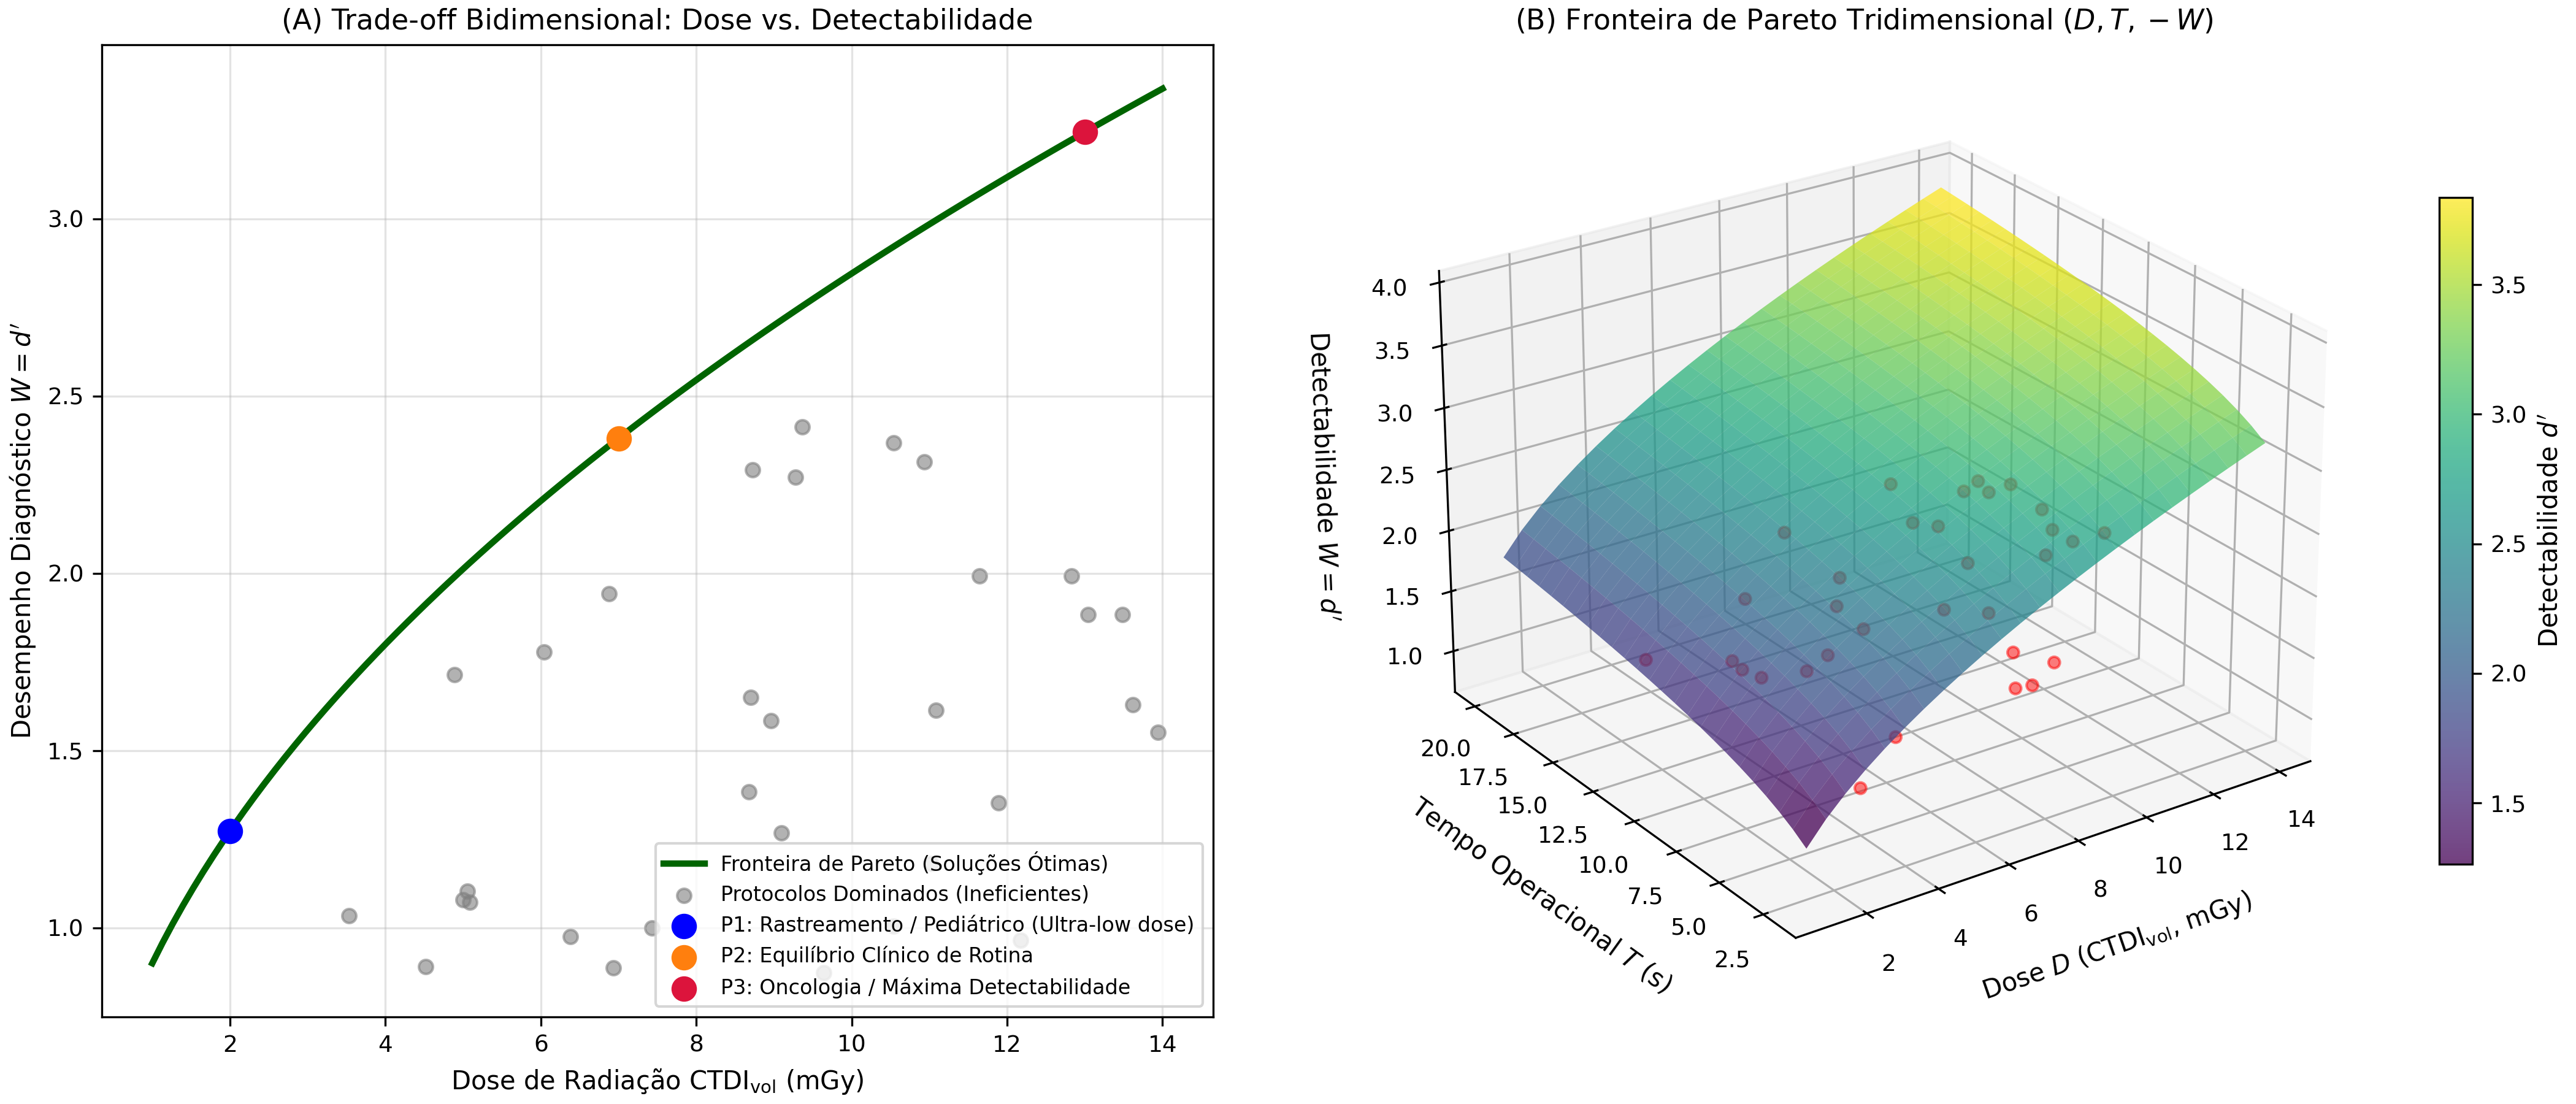
\includegraphics[width=0.98\textwidth]{figuras/fig5_dlmo_pareto_3d.png}
  \caption{Otimização Multiobjetivo em Tomografia Computadorizada e Fronteira de Pareto. (A) Trade-off bidimensional entre Dose e Detectabilidade, ilustrando soluções ótimas na fronteira e protocolos dominados ineficientes. (B) Fronteira de Pareto Tridimensional $(D, T, -W)$, integrando Dose de Radiação ($D$), Tempo Operacional total ($T$) e Detectabilidade Diagnóstica ($W = d'$).}
  \label{fig:pareto_3d}
\end{figure}

O mapeamento dessa superfície de soluções não-dominadas é realizado através do Algoritmo Genético NSGA-II acoplado ao método de tomada de decisão multicritério TOPSIS, permitindo escolher o protocolo ótimo para cada perfil institucional (pediátrico de ultrabaixa dose, emergência ultrarrápida ou oncologia de alta resolução).

\chapter{Arquitetura Computacional, Metrologia Experimental e Aspectos Éticos}
\label{chap:arquitetura_metrologia}

\section{Arquitetura de Software do Pipeline Integrado de Metrologia}
\label{sec:software_arch}

A infraestrutura computacional deste trabalho foi concebida de forma modular em linguagem Python (utilizando NumPy, SciPy, PyDICOM e PyTorch), integrada aos pipelines do grupo GDRFM-IFUSP, conforme detalhado no \cref{fig:software_flow} \cite{choopani2023}.

\begin{figure}[htbp]
  \centering
  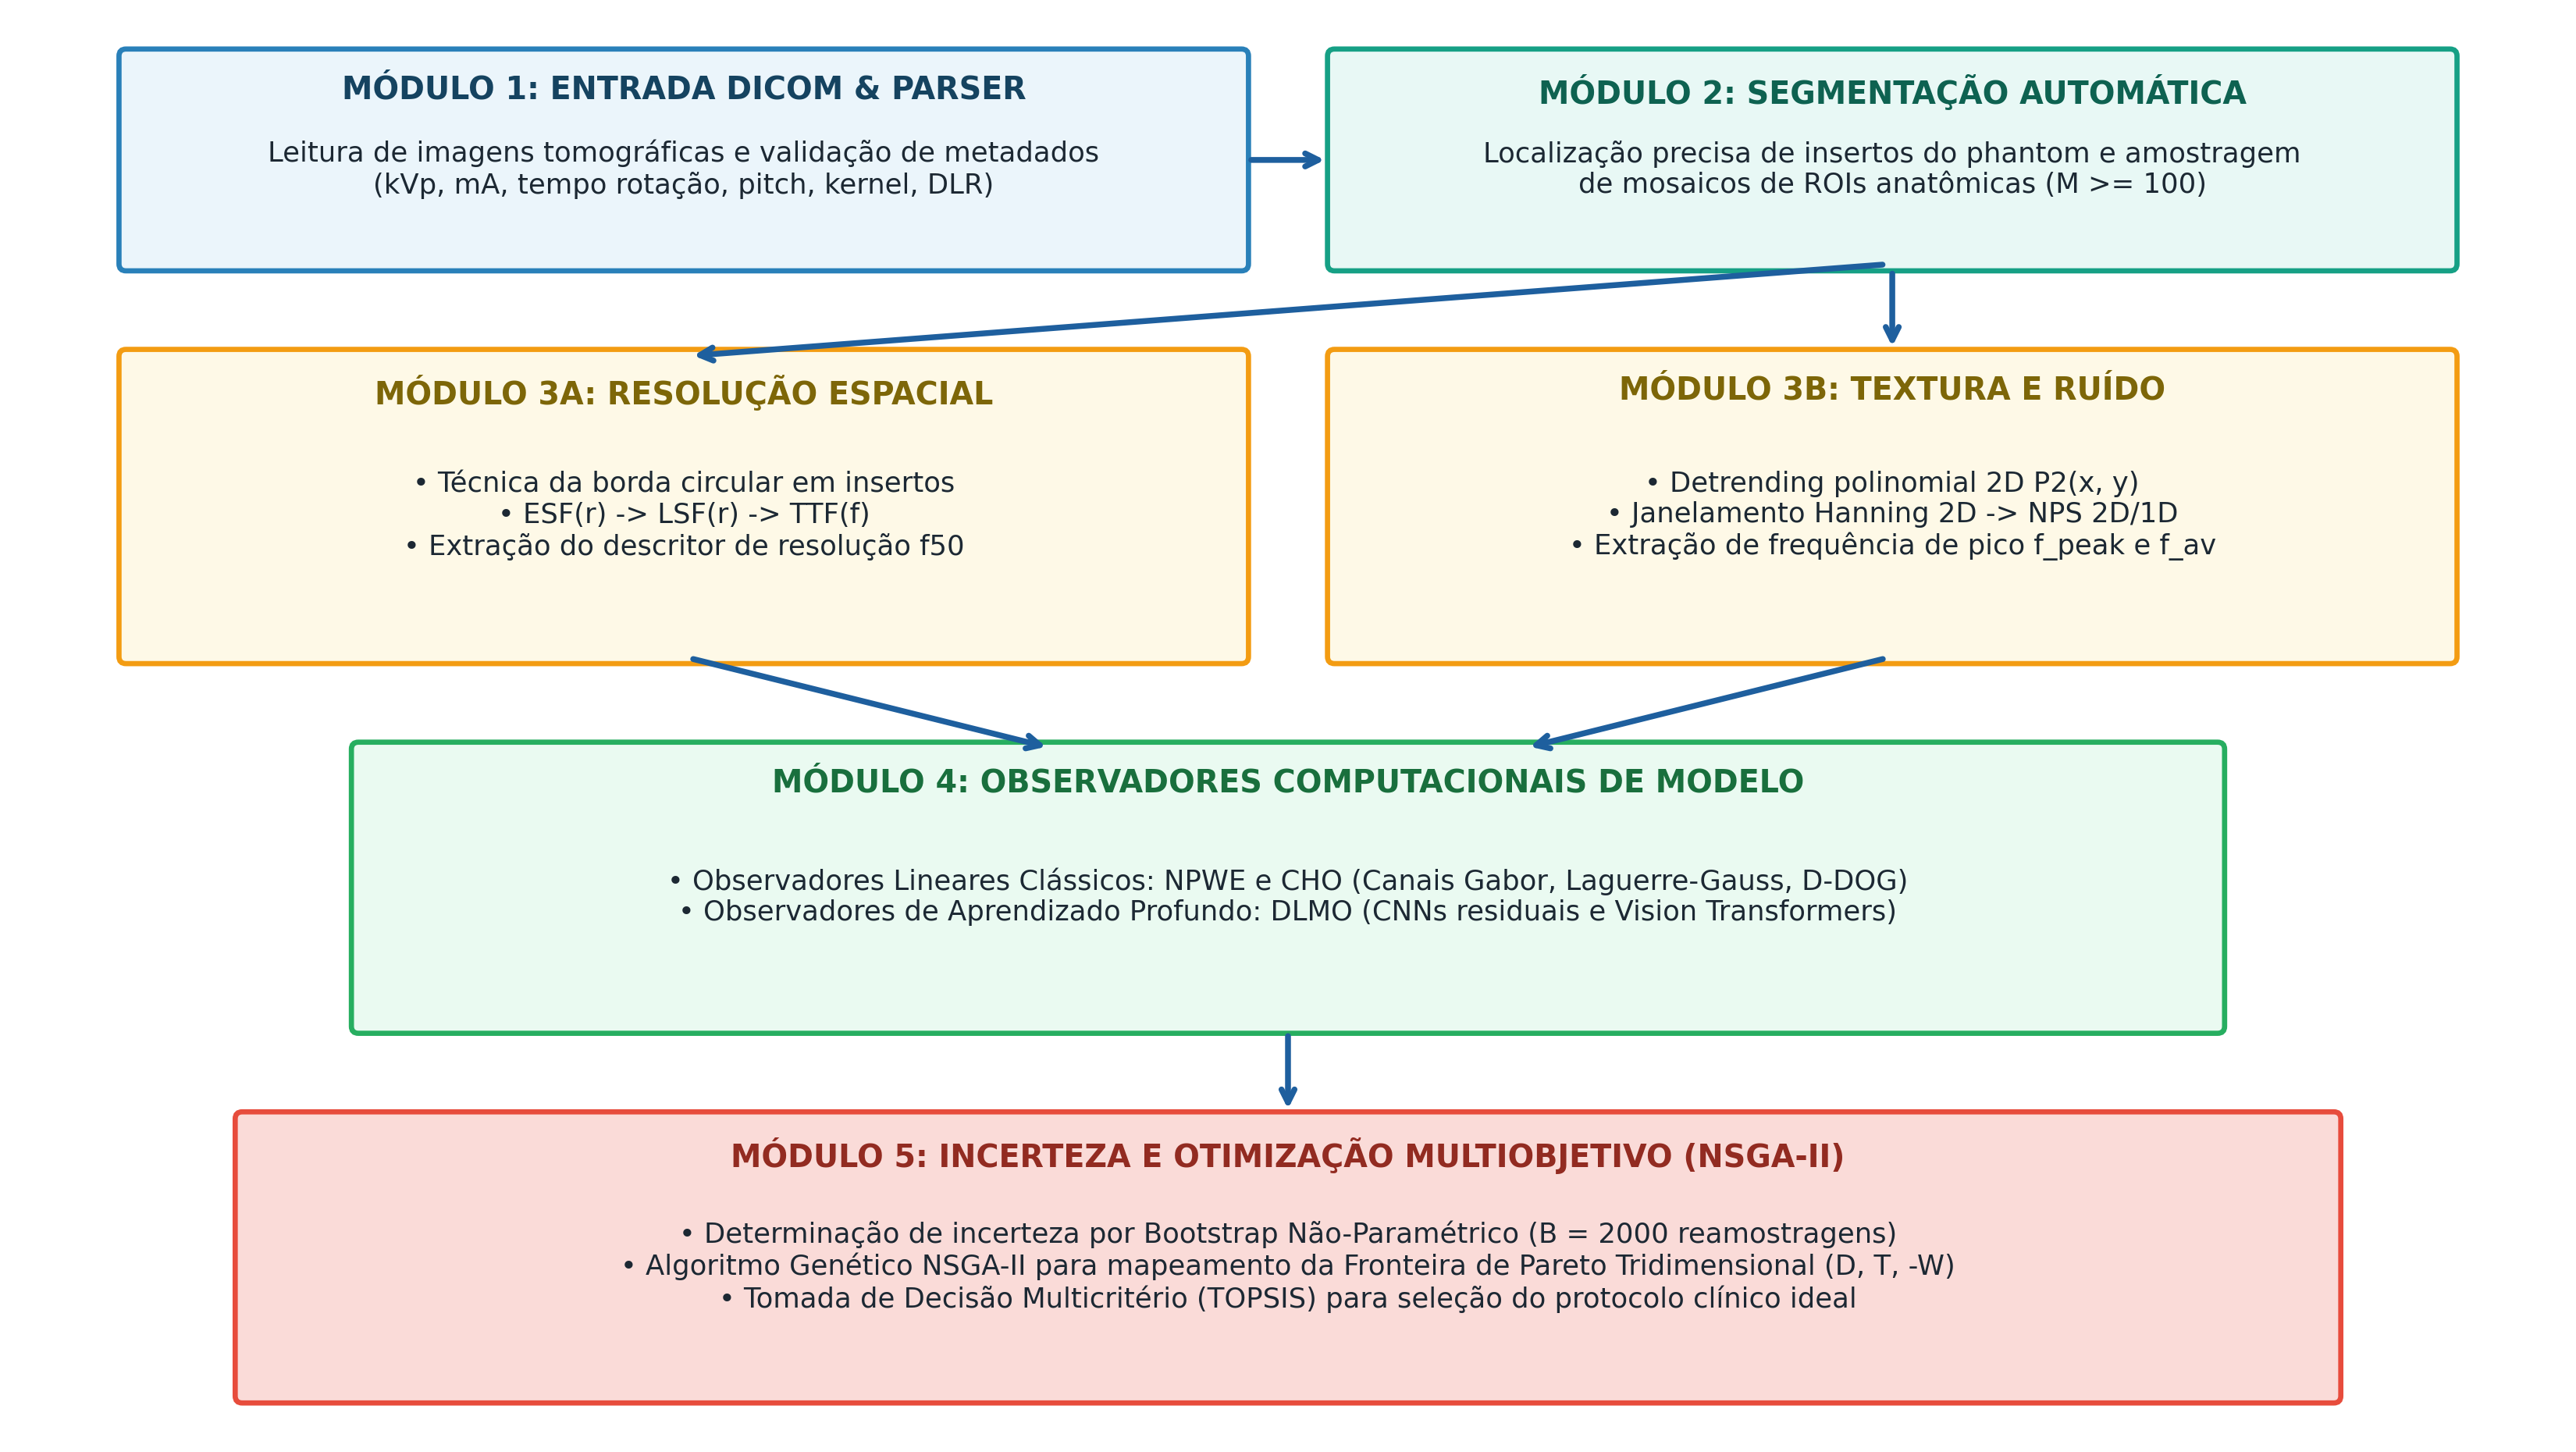
\includegraphics[width=0.95\textwidth]{figuras/flow6_software_pipeline.png}
  \caption{Arquitetura Modular do Software de Metrologia em Tomografia Computadorizada (Pipeline Integrado GDRFM-IFUSP).}
  \label{fig:software_flow}
\end{figure}

O software é composto por cinco módulos encadeados:
\begin{itemize}
  \item \textbf{Módulo 1:} Parser DICOM e validação de metadados de aquisição;
  \item \textbf{Módulo 2:} Segmentação automática dos insertos de calibração e amostragem de mosaicos com $M \ge 100$ ROIs independentes;
  \item \textbf{Módulo 3A:} Cálculo da resolução espacial da tarefa ($ESF \to LSF \to TTF \to f_{50}$);
  \item \textbf{Módulo 3B:} \emph{Detrending} polinomial 2D e cálculo do espectro de ruído ($NPS(u, v)$ e $NPS(f)$);
  \item \textbf{Módulo 4:} Cálculo da detectabilidade via observadores lineares (NPWE e CHO) e modelos por aprendizado profundo (DLMO);
  \item \textbf{Módulo 5:} Análise de incerteza por Bootstrap e otimização da Fronteira de Pareto 3D via algoritmo NSGA-II e método TOPSIS.
\end{itemize}

\section{Protocolo Metrológico Padronizado segundo o Relatório AAPM TG-233}
\label{sec:protocolo_tg233}

As aquisições tomográficas para calibração seguem as diretrizes internacionais da AAPM \cite{aapm_tg233_2019}:
\begin{itemize}
  \item Matriz de imagem de $512 \times 512$ pixels com FOV ajustado ao diâmetro do simulador ($200 \text{ a } 350 \text{ mm}$);
  \item Espessuras de corte de $0{,}5 \text{ a } 1{,}0 \text{ mm}$ para alta resolução e $2{,}5 \text{ a } 5{,}0 \text{ mm}$ para rotina clínica;
  \item Tensões de tubo de 80, 100, 120 e 140 kVp, cobrindo doses de $\text{CTDI}_{\text{vol}}$ de $0{,}5 \text{ mGy}$ a $15 \text{ mGy}$;
  \item Modelagem de lesões esféricas padronizadas com diâmetros de 3, 5, 8 e 10 mm e contrastes clínicos de $-600 \text{ HU}$ (nódulo subsólido pulmonar), $+100 \text{ HU}$ (nódulo sólido hiperatenuante) e $+30 \text{ HU}$ (lesão hepática de baixo contraste).
\end{itemize}

\section{Aspectos Bioéticos, Regulatórios e Desenho Experimental com Seres Humanos}
\label{sec:bioetica}

A condução dos testes psicofísicos 2AFC com médicos radiologistas para obtenção dos dados de calibração exige aprovação formal em Comitê de Ética em Pesquisa (CEP/CONEP):
\begin{itemize}
  \item Recrutamento de no mínimo 20 médicos radiologistas com título de especialista pelo CBR para cada anatomia clínica avaliada ($\ge 60$ leitores no total para tórax, abdome e crânio);
  \item Aplicação obrigatória de Termo de Consentimento Livre e Esclarecido (TCLE) com garantia de anonimização dos dados de desempenho individual;
  \item Monitores diagnósticos com luminância calibrada segundo o padrão DICOM GSDF ($\ge 400 \text{ cd/m}^2$) e iluminação ambiente controlada ($< 15 \text{ lux}$);
  \item Mitigação de fadiga visual através de sessões curtas com no máximo 100 a 150 pares de imagens 2AFC por sessão (duração inferior a 25 minutos).
\end{itemize}

\chapter{Considerações Finais e Perspectivas}
\label{chap:conclusoes}

\section{Síntese da Trajetória Biofísica e Metrológica}
\label{sec:sintese_biofisica}

A trajetória da avaliação da qualidade de imagem em tomografia computadorizada reflete a constante superação de abstrações matemáticas lineares simplificadas em direção à modelagem da complexidade biofísica:
\begin{enumerate}
  \item \textbf{A Fase Linear Analítica (1950--1990):} Partiu da teoria de detecção de sinais e do Observador Ideal Bayesiano, introduzindo filtros oculares (NPWE) para simular as limitações fisiológicas humanas em fundos uniformes;
  \item \textbf{A Modelagem Cortical (1990--2015):} Desenvolveu o Observador de Hotelling Canalizado (CHO), utilizando canais de frequência inspirados na arquitetura do córtex visual primário para superar o ruído estrutural de fundos anatômicos;
  \item \textbf{A Ruptura da Linearidade (2015--2026):} A introdução clínica de algoritmos de reconstrução por aprendizado profundo (DLR) quebrou as premissas de invariância espacial e estacionariedade, expondo os limites dos modelos analíticos tradicionais;
  \item \textbf{O Paradigma da Inteligência Artificial Perceptual e Otimização Multiobjetivo (2026+):} A emergência dos observadores computacionais por aprendizado profundo com mecanismos de auto-atenção (DLMO), calibrados diretamente contra a percepção de radiologistas e integrados a espaços de decisão tridimensionais $(D, T, -W)$.
\end{enumerate}

\section{Impacto Clínico, Operacional e Normativo}
\label{sec:impacto_clinico}

A consolidação dessas ferramentas computacionais produz impacto prático imediato:
\begin{itemize}
  \item \textbf{Segurança Radiológica Personalizada:} Comprova cientificamente que reduções expressivas de dose preservam a detectabilidade diagnóstica de lesões clínicas sutis;
  \item \textbf{Auditoria e Comissionamento Hospitalar:} Fornece rotinas automatizadas para que serviços de física médica realizem auditorias em conformidade com o relatório AAPM TG-233 e com o sistema internacional IAEA 5-Star \cite{iaea_5star_2026};
  \item \textbf{Harmonização de Parques Tecnológicos:} Permite equalizar o desempenho diagnóstico entre tomógrafos de diferentes fabricantes e gerações tecnológicas.
\end{itemize}

\section{Articulação com a Pesquisa de Doutorado Direto (FAPESP 2026--2030)}
\label{sec:fapesp_doutorado}

Esta monografia de conclusão de curso cumpre o papel fundamental de consolidar o embasamento teórico, biofísico, matemático e computacional que sustenta o projeto de pesquisa de Doutorado Direto do autor (FAPESP 2026--2030) no Grupo de Dosimetria e Radioproteção em Física Médica do IFUSP:

O trabalho articula-se com os avanços em PCCT da Dra. Elsa Pimenta (Doutorado 2026) \cite{pimenta2026} e com o pipeline de automação linear no tórax de Davi Amaral (Mestrado FAPESP), estabelecendo as seguintes metas para a tese de doutorado:
\begin{enumerate}[label=\alph*)]
  \item Treinamento e validação experimental do observador DLMO baseado em \emph{Vision Transformers};
  \item Execução do estudo psicofísico nacional 2AFC com mais de 60 radiologistas especialistas sob modelagem ANOVA MRMC;
  \item Validação cruzada de transferibilidade inter-scanners (\emph{leave-one-scanner-out}) em sete tomógrafos de quatro fabricantes distintos no InRad-HCFMUSP e Radboudumc;
  \item Mapeamento experimental completo da Fronteira de Pareto Tridimensional $(D, T, -W)$ para os principais protocolos tomográficos de crânio, tórax e abdome em sistemas EICT e PCCT.
\end{enumerate}

Conclui-se, assim, este trabalho acadêmico com a convicção de que a física médica brasileira continua contribuindo para a vanguarda científica internacional, unindo o rigor analítico da física à missão de preservar vidas humanas.


% ==============================================================================
% ELEMENTOS PÓS-TEXTUAIS (REFERÊNCIAS)
% ==============================================================================
\bibliographystyle{plain}
\bibliography{references}

\end{document}
